\documentclass[12pt]{extreport}
\usepackage[utf8]{inputenc}
\usepackage[english]{babel}
\usepackage[T1]{fontenc}
\usepackage{graphicx, color}
\usepackage{float}
\usepackage{subcaption}
\usepackage{url}
\usepackage{amsfonts}
\usepackage{amsmath}
\usepackage[a4paper,margin=2cm]{geometry}
\usepackage[authoryear]{natbib}
%\usepackage{refcheck}
\usepackage{hyperref}
\hypersetup{
    colorlinks,
    citecolor=black,
    filecolor=black,
    linkcolor=black,
    urlcolor=black
}

\DeclareMathOperator*{\argmin}{arg\,min}

\begin{document}

\begin{titlepage}

\newcommand{\HRule}{\rule{\linewidth}{0.5mm}} % Defines a new command for the horizontal lines, change thickness here
\center % Center everything on the page
 
%----------------------------------------------------------------------------------------
%	HEADING SECTIONS
%----------------------------------------------------------------------------------------


\includegraphics[width=\linewidth]{assets/logos/uvaENG.eps}\\[2.5cm]
\textsc{\Large MSc Artificial Intelligence}\\[0.2cm]
\textsc{\Large Master Thesis}\\[0.5cm]

%----------------------------------------------------------------------------------------
%	TITLE SECTION
%----------------------------------------------------------------------------------------

\HRule \\[0.4cm]
{ \huge \bfseries Detecting and Addressing Change in Machine Learning Data Pipelines}\\[0.4cm] % Title of your document
\HRule \\[0.5cm]
 
%----------------------------------------------------------------------------------------
%	AUTHOR SECTION
%----------------------------------------------------------------------------------------

by\\[0.2cm]
\textsc{\Large Bogdan Floris}\\[0.2cm] %you name
12140910\\[1cm]


%----------------------------------------------------------------------------------------
%	DATE SECTION
%----------------------------------------------------------------------------------------

{\Large \today}\\[1cm] % Date, change the \today to a set date if you want to be precise

Number of credits: 48 ECTS\\ %
November 2019 - July 2020\\[1cm]%

%----------------------------------------------------------------------------------------
%	COMMITTEE SECTION
%----------------------------------------------------------------------------------------
\noindent
\begin{minipage}[t]{0.4\textwidth}
\begin{flushleft} \large
\emph{Supervisors:} \\
prof. dr. Paul \textsc{Groth}\\
Jakub \textsc{Zavrel}
\end{flushleft}
\end{minipage}
\begin{minipage}[t]{0.4\textwidth}
\begin{flushright} \large
\emph{Assessor:} \\
prof. dr. Paul \textsc{Groth}\\
\end{flushright}
\end{minipage}\\[2cm]

%----------------------------------------------------------------------------------------
%	LOGO SECTION
%----------------------------------------------------------------------------------------

%\framebox{\rule{0pt}{2.5cm}\rule{2.5cm}{0pt}}\\[0.5cm]
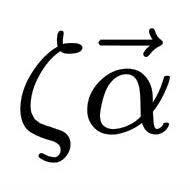
\includegraphics[width=2.5cm]{assets/logos/zeta-alpha-logo.jpg}\\ % Include a department/university logo - this will require the graphicx package
\textsc{\large Zeta Alpha Vector}\\[1.0cm] % 
 
%----------------------------------------------------------------------------------------

\vfill % Fill the rest of the page with whitespace

\end{titlepage}

\chapter*{Abstract}

Insert abstract here.

\chapter*{Acknowledgements}

Insert the acknowledgements here.

\tableofcontents

\listoffigures

\listoftables

\chapter{Introduction} \label{sec:intro}

\begin{itemize}
    \item General introduction to the field (Machine Learning, NLP)
    \item Small overview of the topic being researched in this paper
    \item Why this topic?
    \item Description of the framework \ref{fig:framework}
\end{itemize}

\begin{figure}[h!]
\centering
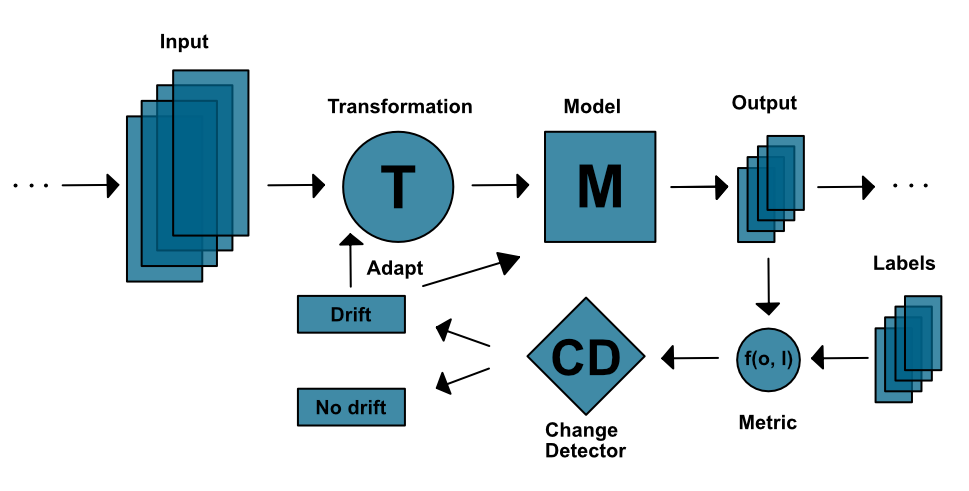
\includegraphics[width=\linewidth]{assets/introduction/framework.png}
\caption{General overview of the architecture}
\label{fig:framework}
\end{figure}

\section{Research Questions}

The main goal of this thesis is to develop a general framework in which machine learning models that are part of streaming data pipelines can detect changes in their output distribution and adapt to them accordingly, while also successfully applying this framework on a specific natural language processing use case that is of interest to Zeta Alpha Vector. This comprehensive topic will be tackled with the following research questions, covered below together with a short description for each question.

\paragraph*{How can we quickly detect that the output distribution of a model has changed given a continuous stream of data, and then report on the degree of change?} Insert description of this research question

\paragraph*{Given that a change was detected, how can we adapt the model efficiently such that the performance is the same as it previously was before the change?} Insert overall description of the question here, them break it down to the two other questions:
\begin{itemize}
    \item \emph{Given a small change (gradual drift or small abrupt drift), can we adapt the model by feeding it with a few examples, compared to retraining it from scratch?} Description about this subquestion.
    \item \emph{Given a big change (big abrupt drift), can we adapt the model by finding a mapping between the old outputs and the new ones which is less expensive to compute than retraining the model from scratch?} Description about this subquestion
\end{itemize}

\chapter{Background}

In this chapter, we introduce the background needed to support the work done in this thesis. First, we give a brief overview of the framework in which change can occur, a data pipeline, and present the concept of online learning. Then we go into more details about the work that has been done on detecting change in this framework, explaining concept drift. Finally, we also present a small overview of the agent of change that acts of the pipeline, word embeddings.

\section{Streaming Data Pipelines and Online Learning}

Since the turn of the century, as memory became increasingly cheaper and the internet more and more widespread throughout the world, companies have started to collect enormous amounts of data. According to \cite{big-data-beginning-future}, the amount of data doubles every two years, with the trend showing no signs of stopping. This phenomenon has given birth to the field of big data, which aims to develop techinques to process and analyze data that is too large or complex for traditional data analysis tools (\cite{wiki:big-data}). Big data has been forcing companies to slowly move away from traditional machine learning algorithms because these work in an offline setting. In offline machine learning, all data is available from the start and can be fed as batches to train the model, with each sample being used more than once potentially. This method is usually infeasible in the context of big data, so \cite{advances-knowledge-discovery} have proposed a few requirements for these large scale machine learning data pipelines:

\begin{itemize}
    \item The training of a model should be done continuously and only on blocks of data or separate samples.
    \item Each sample should only be used once to train the model.
    \item We should assume that the samples are not stored after they have been seen by the model.
\end{itemize}

The third requirement can be relaxed in practice depending on how much storage is available, and most large scale data pipelines usually store at least a recent window of the data.

Online learning is the type of data analysis usually deployed in streaming data pipelines and is defined as a learner which attemps to solve an online decision task by fitting a model to a sequence of data that arrives one at a time (\cite{onlinelearning}). This is in contrast to offline (batch) machine learning, which requires that all data be present when training the model. The main advantage of online learning is that it is highly scalable in terms of both computing power and storage, which is suitable for big data, but it is also not as performant as batch learning since it only sees the samples once and not in an arbitrary order. According to \cite{onlinelearning}, there are three types of online learning:

\begin{itemize}
    \item Supervised online learning where feedback is immediately available.
    \item Online learning with limited feedback (e.g. only a few samples also have labels).
    \item Unsupervised online learning where there is no feedback.
\end{itemize}

The work done in this thesis will mainly focus on supervised online learning, while briefly touching on how a lack of supervision could be handled.

\section{Concept drift} \label{concept-drift}

This section will present a brief introduction to the concept drift phenomenon in machine learning, mention how concept drift can act on data and on the models which were trained on the data, and present some work that has been done into concept drift detection algorithms.

\subsection{Definition}

Online data pipelines should in theory operate endlessly after being deployed, but the nature of data in general makes the environment in which they operate dynamic. One example would be the change in the distribution of the data samples that arrive at the pipeline. This phenomenon is known in theory as concept drift (\cite{survey-concept-drift}). Take for example a set of data $X$ with a target variable $y$, where we are trying to learn a function $f$, such that $y = f(X)$. Predictions models usually require and assume stationarity in the data (\cite{Heng_Wang_2015}), so if we make this assumption we can fit $f$ once and assume that it works for all subsequent data coming to the pipeline. In practice, however, it might happen that the distribution of $X$ changes, and so the relationship between $X$ and $y$ also does, which makes our estimate of $f$ outdated.

We can use the framework (\ref{fig:framework}) to formally define the problem addressed in this thesis as a concept drift issue. Let $W$ be the initial, unprocessed dataset (which will be described in \ref{wos}) with labels $\mathbb{C}$ that denote classes, $\mathbb{T}$ a set of transformation functions (for example a function that extracts features out of the initial dataset), and $X$ the transformed input $\forall i: x_i = t(w_i)$, where $t \in \mathbb{T}$. We can then use Bayesian Decision Theory (\cite{pattern-classification}) to state the classification task. The probability $P(c_k), c_k \in \mathbb{C}$ is known as the \emph{a priori} and reflects the probability that a sample belongs to class $c_k$. The probability $P(X|c_k)$ is known as the \emph{class conditional density function} and reflects the probability density of $X$ when class $c_k$ is known. When can use Bayes' Rule (\cite{bayesrule}) to solve for the \emph{posterior}:

\begin{equation}
    P(c_k|X) = \frac{P(X|c_k) P(c_k)}{P(X)}
\end{equation}

Concept drift occurs if for two time points $t_1$, $t_2$, where $t_2 > t_1$, $\exists x \in X: P_{t_1}(x|c_k) \neq P_{t_2}(x|c_k)$. For our purposes, we will assume that $W$ remains stationary and the distribution shift happens because of a change in the transformation functions $\mathbb{T}$, induced by the pipeline switching from a transformation function to another.

\subsection{Concept drift types}

Concept drift is the shift in the distribution of the dataset as samples come to the pipeline, but of equal importance to both detection and overcoming change is the type of concept drift. \cite{survey-concept-drift} describe a few types of drift, but for all intents and purposes, we can distinguish between three types:

\begin{itemize}
    \item Big abrupt concept drift (figure \ref{fig:big-abrupt-drift}), which is signalled by a big instant change in the distribution that results in the model's accuracy degrading heavily.
    \item Small abrupt concept drift (figure \ref{fig:small-abrupt-drift}), which is signalled by a small instant change in the distrbution that results in the model's accuracy degrading just slighly.
    \item Gradual concept drift (figure \ref{fig:gradual-drift}), which is is signalled by small incremental changes in the distribution that in time have the same effect on the model as a big abrupt change but take a much longer time to occur.
\end{itemize}

\begin{figure}[ht!]
\centering
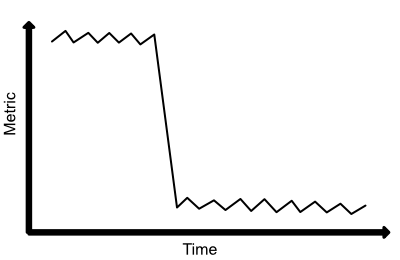
\includegraphics[width=0.6\linewidth]{assets/preliminaries/big-abrupt-drift.png}
\caption{Big abrupt concept drift}
\label{fig:big-abrupt-drift}
\end{figure}

\begin{figure}[ht!]
\centering
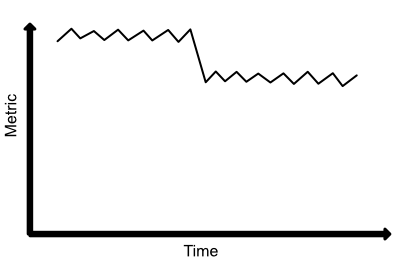
\includegraphics[width=0.6\linewidth]{assets/preliminaries/small-abrupt-drift.png}
\caption{Small abrupt concept drift}
\label{fig:small-abrupt-drift}
\end{figure}

\begin{figure}[ht!]
\centering
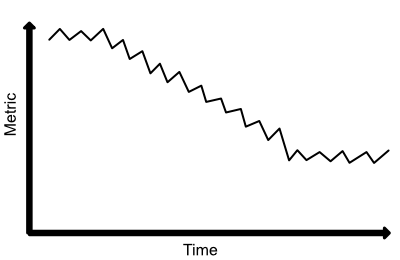
\includegraphics[width=0.6\linewidth]{assets/preliminaries/gradual-drift.png}
\caption{Gradual concept drift}
\label{fig:gradual-drift}
\end{figure}

As mentioned earlier, the type of concept drift encountered has an impact of both detecting and addressing change. As emphasized in the next section, there are quite a few algorithms that are used in practice to detect concept drift, and most of them are better at detecting a specific type of drift, so there is no free lunch. As shown in the experiments in the next chapter, gradual drift is harder to detect and it's quite easy to trigger a false positive. When in comes to addressing change, there are again a few options from which to choose. For example, a fine tuning approach might work for a small abrupt drift, but doing it for a big abrupt drift is akin to retraining the model from scratch, something we would like to avoid.

\subsection{Concept drift detection algorithms} \label{sec:cda}

While there has been ample research involved in detecting anomalies in data which is at rest (\cite{survey-outlier-detection} provides a nice overview of the methodologies employed in anomaly detection and \cite{there-and-back-again} comes with a data mining perspective on outlier detection), machine learning pipelines are anything but static. Data is continuously pushed through the system, so the metrics computed from the models’ outputs are adjusted endlessly. Moreover, this uninterrupted flow in the system makes storing all these metrics infeasible, so the pipeline must be able to make a decision on whether or not a concept drift occurred based only on the most recent samples.

\cite{detecting-change-in-data-streams} wrote one of the pioneering papers on detecting change in data streams and came up with a novel solution that keeps two windows for the incoming stream and comapres the two using a new distance metric that proves to be a good indicator for the degree of change, as it was specifically designed with this in mind. Their method could be improved by using a different method for saving samples, like the space saving algorithm for detecting heavy hitters, as described in \cite{hierarchical-heavy-hitters}. \cite{onlineanomalydetection} uses more simple distance metrics like relative entropy and Pearson correlation, but the approach is tailored towards big data streams. ADWIN (\cite{adwin}) improves on \cite{detecting-change-in-data-streams} by making the size of the window adaptable, resizing it according to the rate of change observed from the data in the window itself. Two methods that are especially suited for detecting drift in classification tasks using metrics are DDM (\cite{ddm}) and EDDM (\cite{eddm}). Both of them are based on the estimated distribution of the distances between classification errors, but DDM is more suitable for abrupt drift, while EDDM is better for gradual drift. A more state of the art paper, \cite{hht}, presents a novel framework for hierarchical hypothesis testing, a concept drift detector named Hierarchical Linear Four Rates, which achieves great results on type I and II errors.

\subsection{Concept drift adaptation}

Concept drift adaptation is a newer topic of interest in the scientific community, but it is gaining more and more traction as models are becoming increasingly costly to retrain. \cite{hht} mentions that there are two different approaches to address concept drifts in streaming data. Continuing adaptation doesn’t include a concept drift detector, but assumes that the environment will change and either keeps updating the model parameters incrementally (\cite{adwin}), or learns an ensemble of models on different windows in the stream (\cite{incremental-learning-of-concept-drift}). Adaptation with drift detection actually employs a detector, which signals that a change has occurred and then makes a decision on which adaption technique to use based on the degree of change (\cite{concept-drift-detection-for-streaming-data}).

\section{Word embeddings} \label{sec:word-embeddings}

We have mentioned in section \ref{concept-drift} that there is a set of transformation functions $\mathbb{T}$ that act as the agent of change on the initial dataset. The transformation agents that will be the main study of this thesis will be word embeddings, which have been main driving force behind the improvements in natural language understanding in the past decade (\cite{word-embedding-survey}). There were two main reasons that necessitated the development of word embeddings to represent text data:

\begin{itemize}
    \item Solutions before the introduction of word embeddings were based on bag of words, where a word was represented by the number of times it appeared in the text. The bag of words method had the clear disadvantage that it produced huge and sparse vectors, which were unsuitable for models. Word embeddings, on the other hand, produce short and dense vectors, which improves both the computational complexity and the understanding of the text (\cite{word-embedding-survey, word2vec}).
    \item Another issue with previous approaches was that the context of a word was not embedded into its representation in the vector space. Take for example these two sentences: \emph{I am writing in my notebook} and \emph{I am writing in my journal}. \emph{Notebook} and \emph{journal} have similar context and this should ideally be represented in their respective vectors. Their relationship is represented in theory by the cosine similarity (\cite{word2vec}): \begin{align}\text{similarity}(w_1, w_2) = \cos(\theta) = \frac{w_1 \dot w_2}{\lVert w_1 \rVert \lVert w_2 \rVert}\end{align}, where $\theta$ is the angle between the vectors of $w_1$ and $w_2$. The cosine similarity is no taken into account with the previous approaches, but word embeddings are optimized to improve it.
\end{itemize}

The breakthrough paper that introduced word embeddings to both the academic world and the industry was \texttt{word2vec} (\cite{word2vec}), which computes pre-trained word embeddings using a skip-gram model. Since then, the field has brought increasingly more improvements to non-contextual word embeddings, with some examples being \texttt{GloVe} (\cite{glove}) and \texttt{FastText} (\cite{fasttext}).

Recently, since the introduction of \texttt{BERT} (\cite{bert}) and ELMo (\cite{elmo}), the field has shifted to contextual word embeddings, which have brought with them great improvements to the state of art on a multitude of tasks (\cite{bert}). These embeddings are trained using a bi-directional transformer model by conditioning on both the left and right context of a word, thus creating better representations. Moreover, besides these different fundamental approaches to computing embeddings, each one of these approaches has dozens of pre-trained variations on different datasets or of different sizes (\cite{huggingface}). For example, \texttt{BERT} has seen variations that make it faster and cheaper computationally, like \texttt{DistilBERT} (\cite{distilbert}), or variations that make it work better for scientific text, like \texttt{SciBERT} (\cite{scibert}).

The trend is clear here. Every year, more and more papers come out that upend the state of the art and improve the natural language understanding models. The AI Index Report 2019 (\cite{aiindex2019}) mentions that the number of AI papers produced each year has increased by more than 9x since 1996, with a lot of them in the field of NLP. Thus, companies and AI practitioners have to constantly adapt to the new state of the art, plugging in new word representations to keep their models up to end. This ends up costing compute and development time, since the neural network models have become increasingly more complex from year to year as well (\cite{aiindex2019}). A data pipeline would be better if it could detect that a change in word embeddings has occurred and adapt itself to the new embedding space. Our work will focus on training a classification model using \texttt{BERT} (\cite{bert}), and then adapting the model to other embedding spaces, namely \texttt{SciBERT} (\cite{scibert}) and \texttt{DistilBERT} (\cite{distilbert}).

\section{Conclusion}

In conclusion, this chapter gives a brief introduction into the key concepts on which the work done in this thesis builds upon. The research will be done not in the traditional machine learning framework, that of offline learning, but in a more applicable situation of online learning, using a streaming data pipeline. To agent of change that will act on the pipeline will be a switch between different ways of computing word embeddings for text data, and we will be using concept drift detection algorithms for signal a change.

\chapter{Framework}

In this chapter, we will focus on establishing the framework in which the experiments on detecting and addressing change can be conducted. Namely, we will talk about the dataset that was chosen for these experiments and how this dataset was fed into a prototype of a data pipeline. Moreover, it will also be mentioned what models were chosen and how they were trained.

\section{Dataset}

In this section, we will introduce the Web of Science dataset, make a case for its selection and then show how it was repurposed as a stream of data in our pipeline.

\subsection{The Web of Science} \label{wos}

Zeta Alpha Vector is a start-up and R\&D lab that aims to build a platform for the scientific community using state of the art natural language understanding which researchers and practitioners can use to find relevant papers and organize their knowledge. Given this goal, our work here involves the processing of a huge number of scientific papers which can then be explored by our users. This is why we have decided that for the purpose of the research done in this thesis, the best dataset to be used is the Web of Science (\cite{wos}).

The Web of Science is a collection of abstracts that were extracted from scientific papers spanning a lot of different fields (\cite{wos}), which make up the labels (e.g. computer science, psychology). The dataset was designed as a hierarchical classification task, in which the purpose is to guess both the broader domain and a subdomain of the paper (e.g. computer graphics is a subdomain of computer science). Since our purpose in this paper is not to solve the task, but to detect and address change, we will simplify the goal to be multiclass classification and only try to guess the subdomain. The dataset is organized into three versions (table \ref{table:wos}), each version having increasingly more samples, but also labels, thus making the task more difficult.

\begin{table}[ht!]
\centering
\begin{tabular}{|l|l|l|l|}
\hline
Version & Samples & Subdomains & Domains \\ \hline
1       & 5,736   & 11         & 3       \\ \hline
2       & 11,967  & 35         & 7       \\ \hline
3       & 46,985  & 134        & 7       \\ \hline
\end{tabular}
\caption{Web of Science versions}
\label{table:wos}
\end{table}

Again, the purpose of this thesis is not to achieve state of the art on this dataset, so we only need the Web of Science as a framework for our experiments. Thus, we have decided to pick the first version of the dataset to save both time and compute power. This choice should have no impact on the overall results of paper, since training on either of the other two versions would just give us a baseline model with different performance compared to the first version.

\begin{figure}[ht!]
\centering
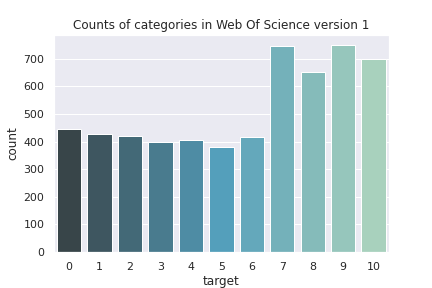
\includegraphics[width=0.8\linewidth]{assets/framework/wos_counts_1.png}
\caption{Web of Science counts for each label}
\label{fig:wos-1}
\end{figure}

We also visualize the distribution of labels in the first version of the Web of Science to check that all classes are represented properlly. \cite{classimbalance} mentions that class imbalance happens when one class outnumbers the others 10 to 1, but we can see from figure \ref{fig:wos-1} that we do not have this problem, and so we can use the usual classification methods and metrics.

\subsection{Data pipeline}

Having chosen an appropriate dataset for our experiments, we now shift our focus to describing the data pipeline that will receive at its point of entry samples from the dataset. This pipeline will mostly follow the diagram shown in figure \ref{fig:framework}.

The first requirement is to pick a suitable framework in which to design the pipeline. While frameworks like \texttt{Kafka} (\cite{kafka}) or \texttt{Flink} (\cite{flink}) are excellent for an industry setting where high performance and scalability are required, they are overkill for the prototype pipeline we are designing. Thus, we have chosen to use \texttt{Scikit-Multiflow} (\cite{skmultiflow}), a data streaming library that builds on top of \texttt{Scikit-Learn} (\cite{sklearn}) and aims to provide the same algorithms as its parent library but adjusted to online learning. The library is a good choice since it allows us to keep the same challenges that come with machine learning in data pipelines in order to make our experiments more robust, but also speed up the implementation time since its API is compatible with \texttt{Scikit-Learn}, the most used machine learning library.

The first step in the pipeline is to pre-process the data, since text tends to contain information that is irelevant to classification (e.g. tags, spaces, punctuation, miss-spellings) (\cite{textclassification}). After cleaning the data, we can then feed it to one of the three chosen transformer (\cite{huggingface}) models (see section \ref{sec:word-embeddings}) and their corresponding tokenizers to extract the word embeddings. To keep everything consistent throughout all experiments, we have chosen to keep the embedding dimension to 768, to cut of all sequences of tokens to 512 if they are longer, to pad everything with zeros if the sequences of tokens are shorter than 512, and to keep the last layer of the transformer models (\cite{attention}) as the inputs to the models. This results in a final dataset that is held in a three-dimensional tensor of shape $(N, 512, 768)$, where $N$ is the number of samples.

The next step of the pipeline is to input these samples to the model (section \ref{sec:models}) to get a predictions that will then be used together with the labels to compute metrics which will be fed to the change detector (chapter \ref{sec:detecting}). The detector can then make a decision on whether or not a change has occurred and alert the system that the change must be addressed (chapter \ref{sec:addressing}).

\section{Models} \label{sec:models}

This section covers the next step in our data pipeline, the models. Two models have been chosen for our experiments: Naive Bayes, which acts as a baseline, and an LSTM that will be the main object of our experiments. The comparison between the two models will be developed in this section and in the subsequent chapters and will serve to highlight how a probabilistic model and a neural network model behave under change. The next two subsections will present a more in depth look at the models (explanation on the methods, training process, etc.), but the important results averaged over 5 runs are shown in table \ref{table:model-metrics}.

\begin{table}[ht!]
\centering
\begin{tabular}{|l|l|l|l|l|l|l|}
\hline
            & Loss & Train Accuracy & Test Accuracy & Precision & Recall & Macro F1 \\ \hline
Naive Bayes & N/A        & 0.612          & 0.554         & 0.575          & 0.571       & 0.567         \\ \hline
LSTM        & 0.087      & 0.955          & 0.898         & 0.894          & 0.895       & 0.892         \\ \hline
\end{tabular}
\caption{Metrics for the Naive Bayes and LSTM models averages over 5 runs (the first 2 columns are on the train set, while the rest are on the test set).}
\label{table:model-metrics}
\end{table}

\subsection{Naive Bayes} \label{sec:nb}

The Naive Bayes classifier is a supervised machine learning algorithm that is quite popular in natural language processing (\cite{naivebayes}) and is usually used as a baseline for other methods in text classification (\cite{nb-baseline}). The algorithm is based on Bayes' Rule (\cite{bayesrule}) and the following equation is used to classify a sample:

\begin{equation}
    P(y|x_1, ..., x_k) = \frac{P(x_1, ..., x_k|y)P(y)}{P(x_1, ..., x_k)}
\end{equation}
, where $x_{1..k}$ are features of a sample and $y$ the label. Since the marginal probability remains equal throughout the computations, we can exclude it. Moreover, the Naive Bayes makes an important assumption that the features of a data point are conditionally independent given the label. Even though this assumption is not corrent more often than not, it turns out that Naive Bayes usually works in practice on simpler classification tasks (\cite{naivebayes}). In fact, a good predictor for the performance of the classifier is the amount of information lost due to the independence assumption, as the experiments in \cite{naivebayes} show.

For our experiments, we use the implementation of Naive Bayes from the \texttt{Scikit-Learn} package, which also supports a \texttt{partial\_fit} method, suitable for online learning, thus making the implementation compatible with our data pipeline. We have mentioned in section \ref{sec:models} that a sample representation in our dataset is a 2D matrix with shape $(512, 768)$, but Naive Bayes only supports samples that are in one dimension. This leaves us with two options: we can either aggregate (taking the average or the maximum) over one of the dimensions, or just flatten matrix. We have found by trying all these methods that flattening the matrix is both more expensive and produces worse results than aggregating. The best performing method was taking the maximum over the first dimension, thus producing a sample of size $768$ that contains all the information of a scientific paper abstract.

These samples were then fed to the data pipeline in batches of $32$ for $10$ epochs in order to train the Naive Bayes classifier, while keeping track of the training set accuracy. At the end of each epoch, we also computed four different metrics (accuracy, precision, recall, and macro F1) on a holdout testing set to make sure that the model was not influenced by a class imbalance problem. The results are shown in table \ref{table:model-metrics} and in figures \ref{fig:nb-acc} and \ref{fig:nb-metrics}.

\begin{figure}[ht!]
\centering
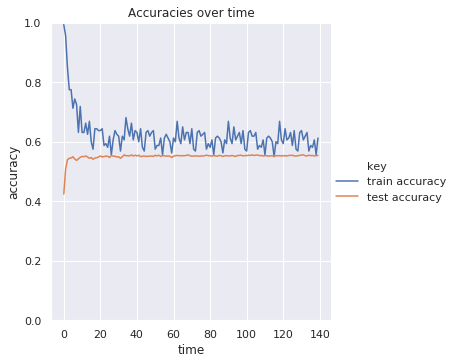
\includegraphics[width=0.8\linewidth]{assets/framework/nb_BERT_accuracy_holdout.png}
\caption{Naive Bayes accuracy over time using BERT embeddings}
\label{fig:nb-acc}
\end{figure}

As we can see for the results, the Naive Bayes method performs decently enough for a multiclass classification problem with 11 classes (the $0.55$ test set accuracy is substantially better than the accuracy of $0.09$ accuracy of a random guesser algorithm). Moreover, we can see from figure \ref{fig:nb-metrics} that class imbalance is not a issue here since all the metrics that we have chosen have almost identical curves. Furthermore, the model converges almost quite fast and the curve shows not oscillations on the test set (figure \ref{fig:nb-acc}), so we can conclude that it is pretty robust on the dataset that it was trained on. However, as we will see in the next chapter (\ref{sec:detecting}), as soon as the features deviate just a little bit, the model performs much worse, so it is not robust to changes in data distribution.

\begin{figure}[H]
\centering
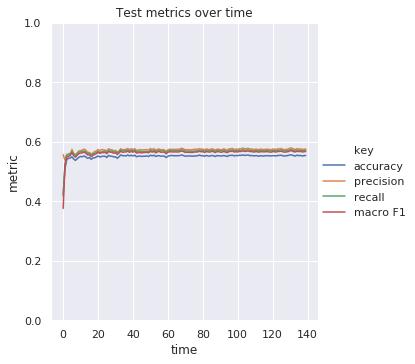
\includegraphics[width=0.8\linewidth]{assets/framework/nb_BERT_test_metrics_holdout.png}
\caption{Naive Bayes metrics over time for the test set}
\label{fig:nb-metrics}
\end{figure}

\subsection{LSTM} \label{sec:lstm}

Long Short Term Memory (LSTM) (\cite{lstm}) network is a type of ANN that has been created to address a major problem with Recurrent Neural Networks (RNNs), that of the vanishing gradient. RNNs were designed to model continuity, meaning that the network could learn from past events. This is especially useful in the context of NLP, where we would like to model problems based on sequences of words. The vanishing gradient problem occurs when there are long-distance relationships between the elements of the sequence. By continuously derivating, the gradient will eventually be 0 and thus we cannot perform a meaningful update. LSTMs are designed specifically to solve this problem, by making small modifications to the information by multiplications and additions through a mechanism called a cell state that allows for information to easily flow through the network (\cite{lstmrnnfundamentals}). Cells make use of three gates that determine what information gets passed along to the next cell (\cite{colahlstm}):

\begin{itemize}
    \item Input gate, which decides how the input will affect the cell state
    \item Forget gate, which decides what information from the previous cell state is kept and what is forgotten
    \item Output gate, which determines the output hidden state that gets sent to the next cell
\end{itemize}

All these properties make LSTMs a very suitable choice as our model with which we can solve the text classification task. Neural network models are already online learning methods by their contruction since they are using gradient descent on batches of an arbitrary number of samples. Thus, we can simply incorporate an LSTM into our data pipeline. The architecture will be kept simple since the task is not overly complex and we would like to save computation time. The network has two LSTM layers with a hidden dimension of $256$ and a final fully connected layer that is used for classification. Unlike the Naive Bayes model, we had no issues feeding the 2D samples to the LSTM layers since the model is specifically designed to handle sequences. However, we encountered a similar issue before feeding the output of the LSTM layers to the fully connected layer for classification. \cite{maxpoolinglstm} mentions that absolute value max pooling over the hidden dimension of the LSTM output will transform the vector to one dimension while preserving the most important information.

As we have done with the Naive Bayes model, we fed the samples to the data pipeline with an LSTM model in batches of $32$ for $10$ epochs, while keeping track of the train set loss and accuracy. We again computed the four metrics mentioned in the previous subsection at the end of each epoch on the test holdout test. The results are shown in table \ref{table:model-metrics} and figures \ref{fig:lstm-loss-acc} and \ref{fig:lstm-metrics}.

\begin{figure}[H]
\centering
\begin{subfigure}{.5\textwidth}
  \centering
  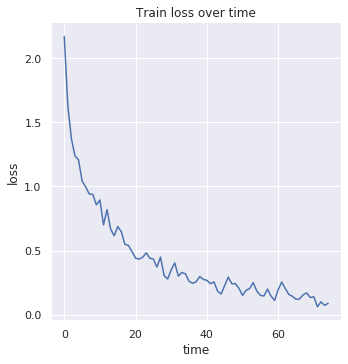
\includegraphics[width=.76\linewidth]{assets/framework/lstm_BERT_loss_holdout.png}
  \caption{Loss over time}
  \label{fig:lstm-loss}
\end{subfigure}%
\begin{subfigure}{.5\textwidth}
  \centering
  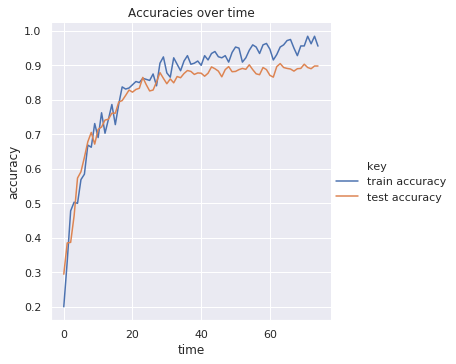
\includegraphics[width=\linewidth]{assets/framework/lstm_BERT_accuracy_holdout.png}
  \caption{Accuracy over time}
  \label{fig:lstm-acc}
\end{subfigure}
\caption{LSTM loss and accuracy over time using BERT embeddings}
\label{fig:lstm-loss-acc}
\end{figure}

As assumed, the results show us that the LSTM is a much better model for text classification since it does not assume independence between the features, but actually tries to learn that dependence. We obtain a test set accuracy of 0.898 averaged over 5 runs and while the model doesn't converge quite as fast as the Naive Bayes, it still manages to arrive at a good performance quite quickly, as can be seen from figure \ref{fig:lstm-loss-acc}. We also obtain the same results about the class imbalance problem as the Naive Bayes, with all four metric curves looking almost identical. The LSTM is not only very robust on the dataset that it was trained on, but as we will show in chapter \ref{sec:addressing}, it can also handle perturbations in its input distribution, with its performance declining much slower than the Naive Bayes model.

\begin{figure}[H]
\centering
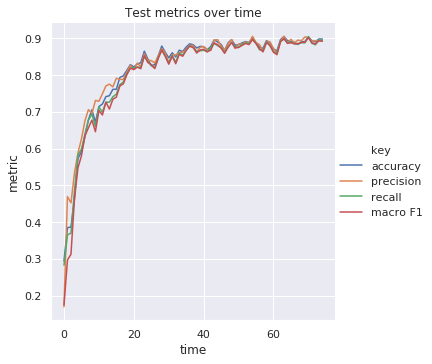
\includegraphics[width=0.8\linewidth]{assets/framework/lstm_BERT_test_metrics_holdout.png}
\caption{LSTM metrics over time for the test set}
\label{fig:lstm-metrics}
\end{figure}

\section{Conclusion}

This chapter presented most of the preliminary work that went into this thesis before actually answering the research questions outlined in the introduction (chapter \ref{sec:intro}). It presents the Web of Science dataset and how it was transformed to a data stream, and then goes on to show how the two models that we have chosen (Naive Bayes and LSTM) were adjusted to our framework and trained, while showing their performance on the Web of Science classification task. Although this was not the purpose of this thesis, we have shown how the two models are quite different in terms of both robustness and performance, with the LSTM displaying great accuracy without any hyper-parameter tuning.

\chapter{Detecting change} \label{sec:detecting}

Now that we have explained the framework in which the experiments in this thesis will be conduced, we can proceed to answer the first research question outlined in chapter \ref{sec:intro}: \emph{How can we quickly detect that the output distribution of a model has changed given a continuous stream of data, and then report on the degree of change?}.

This chapter, and every subsequent chapter after this, will be organized as follows. We will first explain how the experiments were setup and present every important detail in order to better understand the result, which will be shown after. Finally, we will interpret the results in a discussion.

\section{Experimental Setup}

We have outlined a few approaches to drift detection in section \ref{sec:cda}, but there are too many algorithms to try all of them in practice, so we have decided to stick with a few that have proven themselves throughout literature. \cite{mcdiarmid} mention that DDM, EDDM, and ADWIN have been frequently considered as benchmarks, while Page-Hinkley (\cite{pagehinkley}) was a pioneer method in the field. Coincidentally, \texttt{Scikit-Multiflow}, the library on which our pipeline was built, has implementations for all of these algorithms, so we have experimented with all four before deciding on a suitable change detector. As expected, Page-Hinkley did not perform on par with the other three since it's an older method. Both DDM and EDDM are statistical analysis methods which attemp to detect drift based on statistical parameters such as the mean and standard deviation, so in theory they sacrifice detection accuracy for minimal storage and speed. ADWIN, however, is a window based method which needs to store two windows of the data stream, one older and another newer. If there is a significant difference between these two windows, than ADWIN signals a drift. This method is supposed to be more accurate, but it also needs to store two windows of data and compute a difference metric on those two windows, which makes it more computationally expensive. In practice, however, we have found that DDM and ADWIN perform on par on abrupt drift, while EDDM outshines the rest on gradual drift, which makes sense since it was specifically designed for this. Thus, we have decided to use DDM for the abrupt drift experiments, and EDDM for the gradual drift ones.

The experiments will be run as follows: given the models trained in the previous chapter on BERT embeddings, we first push our whole dataset through the pipeline, again transformed using BERT, and evaluate the predictions made by the model against the labels, producing an accuracy. This accuracy will then be inputted to the change detector for each batch that runs through the pipeline. Thus, the change detector can build an accurate mean and standard deviation for the dataset. After the whole dataset is finished, we are now ready to introduce change in the pipeline, by re-running the dataset from the beginning, but now transformed using either one of SciBERT or DistilBERT, or by adding random noise to the BERT embeddings. Again, the predictions will be evaluated against the labels, and the accuracies pushed to the change detector. Note that the detector can signal a warning, meaning that the pipeline is close to deviating from the mean, or an actual drift. The detector will be queried for either a warning or a drift after each batch, both when running the stream the first time (to test that the detector is robust and doesn't signal false positives) and the second time (to detect changes).

The three agents of change were picked for the following reasons:
\begin{itemize}
    \item SciBERT (\cite{scibert}) provides a completely different representation for the documents, since it was training on scientific text. Thus, there should be no correlation between these embeddings and BERT, and so we can introduce SciBERT as an agent of big abrupt drift, a type of change that should be felt instantly by the pipeline and will result in huge degradation to the accuracy of the model.
    \item DistilBERT (\cite{distilbert}), on the other hand, was trained to be a faster and smallert version BERT, while retaining most of its language understanding capabilities. This should mean that models trained on BERT should perform on par when new samples arrive that have been transformed using DistilBERT. We can then introduce this embeddings as an agent of small abrupt drift, which should also be felt instantly by the pipeline, but will result in minimal or no degradation in the performance.
    \item The last agent that we need to introduce needs to be able to simulate a gradual drift. For these experiments, we have to adjust our experiments framework a bit by only running the stream once, but from a specific batch, we start to add random gaussian noise in an increasing fashion as described: we keep the mean of the normal distribution to 0, and we pick a maximum standard deviation. Then, we make an evenly spaced interval of standard deviations between zero and the maximum. We then sample the random noise from the distribution, we thus every batch gets increasingly more noise added to it. Note that we will be running experiments with three maximum standard deviations: $1.0$, $2.0$, and $3.0$.
\end{itemize}

The last point that we need to mention before getting on with showing the actual results is that we previously made an assumption about how we compute the metrics that are being inputted to the change detector. In real world data pipelines, this is however not usually a valid assumption to make since the incoming data to the pipeline is not labelled most of time. This means that we also need to find a way in which to detect change when we have a model, but the data arriving at it does not have labels. One way to do this is to assume that the model in the current pipeline produces perfect predictions and use them as labels to produce metrics against the pipeline with a newly introduced agent of change. As an example, which we will see in the results section, we assume that the BERT embeddings produce perfect predictions (with accuracies of $1.0$), and use those labels to compute metrics with the $SciBERT$ predictions. In practice, however, we have found that only inputting accuracies of $1.0$ to the change detector when running the BERT stream, made the detector too sensitive to any value that wasn't $1.0$. Thus we have decided to actually input random uniform numbers between $0.9$ and $1.0$ to the change detector and also tune its sensitivity down by increasing the threshold when the detector signals a warning or a change.

\newpage

\section{Results}

Now that we have established how the experiments will be run, we can go on to present the results for both models. We will start of with Naive Bayes and then move on to the LSTM. Both of them will have the supervised and unsupervised results shown side by side for better clarity, and the figures will have a consistent format: the blue stream will be the one on which the model was trained (i.e. BERT embeddings), while the green stream will be the stream impacted by change (i.e. SciBERT or DistilBERT). Moreover, warnings outputted by the change detector are visualized by a yellow cross, and the drift by a red cross. Note that for the random noise change detection experiments, there is only one stream, the blue one, which is slowly being impacted by change.

\subsection{Naive Bayes model}

We first change embeddings from BERT to DistilBERT (i.e. simulating small abrupt drift) for both the supervised and unsupervised case and showcase the results in figures \ref{fig:nb-diff-embed-super-B-D} and \ref{fig:nb-diff-embed-unsuper-B-D}. DistilBERT embeddings are supposed to preserve the embeddings space of BERT, but it seems that the Naive Bayes model is fitted very closely to the dataset that it was trained on, and it is not robust to small changes in its inputs. Except for a few outliers, we can see that the performance of the model drops by a lot instantly. The change detector however did its job quite well and outputted a few warnings very fast before finally triggering a drift. Moreover, we can see that the places where the outliers are can be found in both the supervised and the unsupervised variants and thus it seems that our method for computing metrics is working so far. Note however that the change is triggered much faster than in the supervised case, mostly because the supervised case has an average accuracy of about $0.6$, while in the unsupervised case we are inputting to the change detector random numbers between $0.9$ and $1.0$, thus it seems that our proposed method works best when the performance of the model is very good on the dataset on which it was trained on.

\begin{figure}[H]
\centering
\begin{subfigure}{.5\textwidth}
  \centering
  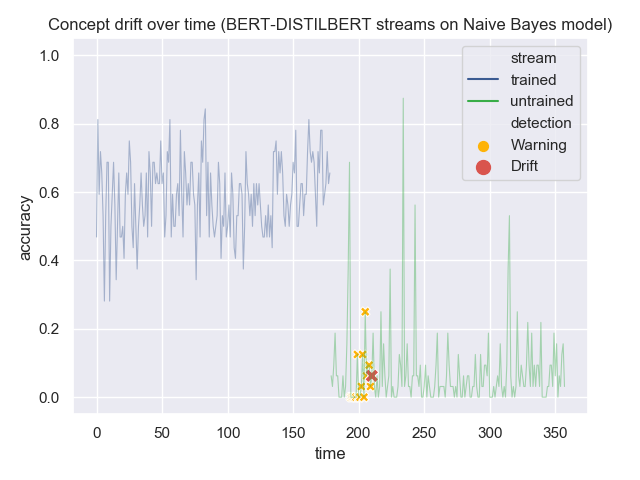
\includegraphics[width=\linewidth]{assets/detecting-change/diff_embed_nb_wos_1_BERT_DISTILBERT.png}
  \caption{Supervised change detection}
  \label{fig:nb-diff-embed-super-B-D}
\end{subfigure}%
\begin{subfigure}{.5\textwidth}
  \centering
  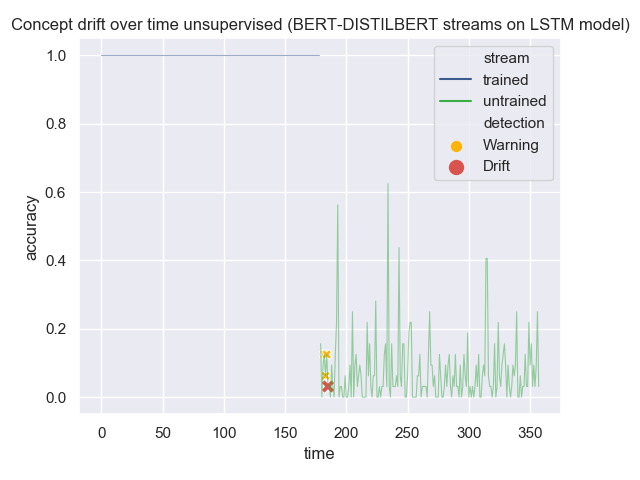
\includegraphics[width=\linewidth]{assets/detecting-change/diff_embed_nb_wos_1_BERT_DISTILBERT_unsupervised.png}
  \caption{Unsupervised change detection}
  \label{fig:nb-diff-embed-unsuper-B-D}
\end{subfigure}
\caption{Detecting change using different embeddings (BERT-DISTILBERT) in the Naive Bayes model}
\label{fig:nb-diff-embed-B-D}
\end{figure}

Figures \ref{fig:nb-diff-embed-super-B-S} and \ref{fig:nb-diff-embed-unsuper-B-S} present the results for the experiments when we are changing from BERT to SciBERT (i.e. simulating big abrupt drift). Given that the previous figures also showed a big change, it is not surprising that these results showcase the same phenomenon. Again, performance degrades instantly, but in this case, we don't even have the outliers in the green stream. This is expected, however, since SciBERT is a completely different embedding from BERT and so the performance should degrade. The change detector also outputs the change quite fast, more so in the unsupervised case, for the reasons explained previously.

\begin{figure}[H]
\centering
\begin{subfigure}{.5\textwidth}
  \centering
  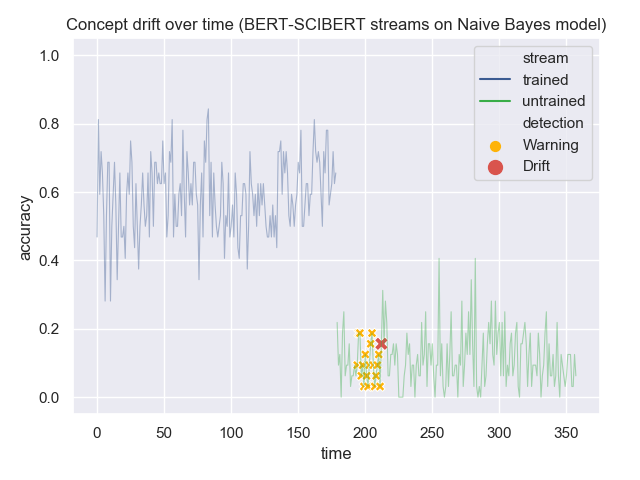
\includegraphics[width=\linewidth]{assets/detecting-change/diff_embed_nb_wos_1_BERT_SCIBERT.png}
  \caption{Supervised change detection}
  \label{fig:nb-diff-embed-super-B-S}
\end{subfigure}%
\begin{subfigure}{.5\textwidth}
  \centering
  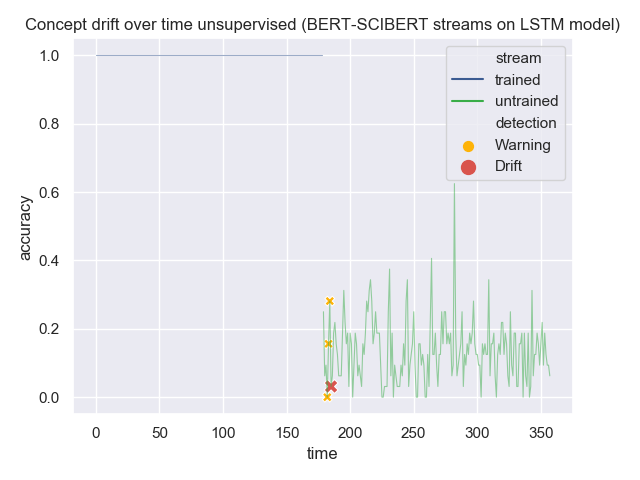
\includegraphics[width=\linewidth]{assets/detecting-change/diff_embed_nb_wos_1_BERT_SCIBERT_unsupervised.png}
  \caption{Unsupervised change detection}
  \label{fig:nb-diff-embed-unsuper-B-S}
\end{subfigure}
\caption{Detecting change using different embeddings (BERT-SCIBERT) in the Naive Bayes model}
\label{fig:nb-diff-embed-B-S}
\end{figure}

Now we can move on the the third agent of change, that is adding random gaussian noise to the BERT embeddings to simulate gradual drift. As explained in the previous subsection, after a few dozen batches, we start adding this noise in increasing fashion by sampling from a normal distribution with mean zero and a standard deviation between 0 and a predetermined maximum. We run this experiments for three maximum standard deviations: $1.0$ (figure \ref{fig:nb-gradual-std-1}), $2.0$ (figure \ref{fig:nb-gradual-std-2}), and $3.0$ (figure \ref{fig:nb-gradual-std-3}). Again, we start to notice the same pattern for the Naive Bayes model, that even slightly small changes to the input distribution results in significant drops in its performance. For the maximum standard deviations of $2.0$ and $3.0$, the drop to the performance of a random guesser is almost instant, with the change detector reacting accordingly. For the standard deviation $1.0$, it takes a few batches for the performance to drop, with the change detector being a little slower as was expected.

\begin{figure}[H]
\centering
\begin{subfigure}{.5\textwidth}
  \centering
  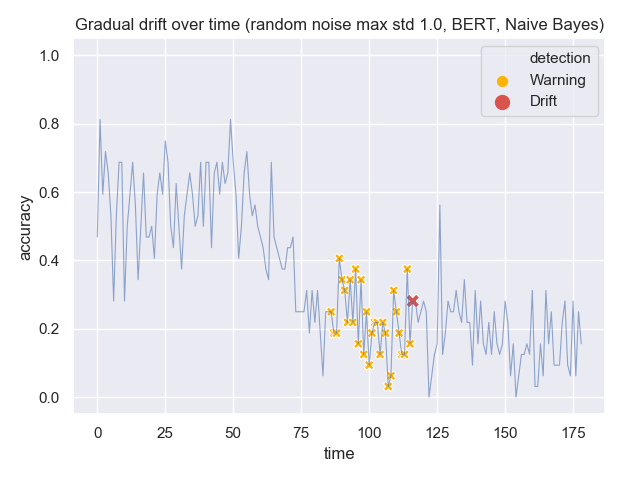
\includegraphics[width=\linewidth]{assets/detecting-change/gradual_noise_random_std_1_nb_wos_1_BERT.png}
  \caption{Gradual with std 1.0}
  \label{fig:nb-gradual-std-1}
\end{subfigure}%
\begin{subfigure}{.5\textwidth}
  \centering
  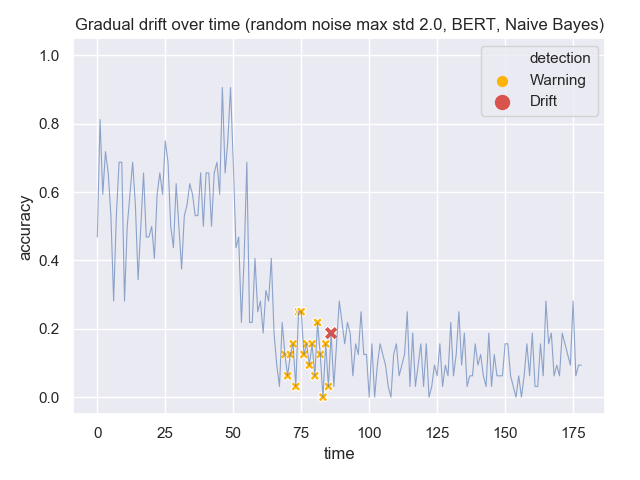
\includegraphics[width=\linewidth]{assets/detecting-change/gradual_noise_random_std_2_nb_wos_1_BERT.png}
  \caption{Gradual with std 2.0}
  \label{fig:nb-gradual-std-2}
\end{subfigure}
\begin{subfigure}{.5\textwidth}
  \centering
  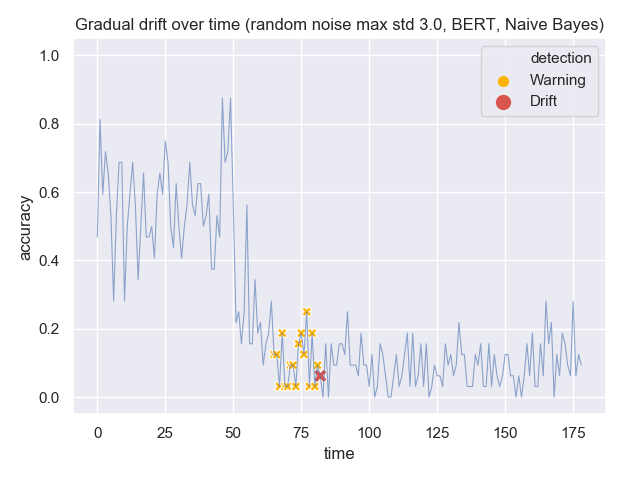
\includegraphics[width=\linewidth]{assets/detecting-change/gradual_noise_random_std_3_nb_wos_1_BERT.png}
  \caption{Gradual with std 3.0}
  \label{fig:nb-gradual-std-3}
\end{subfigure}
\caption{Detecting gradual change by adding random noise with different stds in the Naive Bayes model}
\label{fig:nb-gradual}
\end{figure}

\subsection{LSTM model}

Now that we have shown how the Naive Bayes model behaves under change, we can move on to a more interesting neural network based model which is supposed to provide a much better approximation for the input distribution (i.e. the BERT embeddings space), the LSTM. The results are presented in the same order as in the previous subsection, starting with changing embeddings from BERT to DistilBERT in order to simulate small abrupt drift when we assume labels and when the assumption is not made. These results are shown in figures \ref{fig:lstm-diff-embed-super-B-D} and \ref{fig:lstm-diff-embed-unsuper-B-D} and they confirm our expectations that the LSTM model should behave almost the same when changing from BERT to DistilBERT since they were purposefully designed to be interchangeable. We see from figure \ref{fig:lstm-diff-embed-super-B-D} that the performance only drops slightly when switching streams, since there is only an approximately $0.5$ drop in accuracy on average on the green stream compared to the blue one. Moreover, the change detector correctly stays in the warning zone for a few dozen batches to see if the performance recovers before finally signalling a drift when about half the stream has been run. When labels are not available (figure \ref{fig:lstm-diff-embed-unsuper-B-D}), we see that the green curves in both figures look quite similar so the solution that we have come up with in which we replace the labels with the predictions of the first stream seems to be working quite well. However, since the random accuracies (between $0.9$ and $1.0$) that were fed to the change detector in the unsupervised case are a bit lower on average than the accuracies produced when we do have labels, the detector doesn't consider that the deviation is high enough to signal a drift, so it stays in the warning zone until the end of the stream. This could have been fixed by adjusting the sensitivity of the change detector, but for the purpose of the experiments, we have kept all parameters the same between the experiments. These results show that the DDM detector is robust enough to also detect change that is quite small, and even if it doesn't, it stays in a perpetual warning zone that can help identify drifts nonetheless. One improvement that we could bring to DDM is to also introduce a parameter that controls the length of the warning zone (i.e. if we are in a warning zone for a fixed duration, we signal an actual drift).

\begin{figure}[H]
\centering
\begin{subfigure}{.5\textwidth}
  \centering
  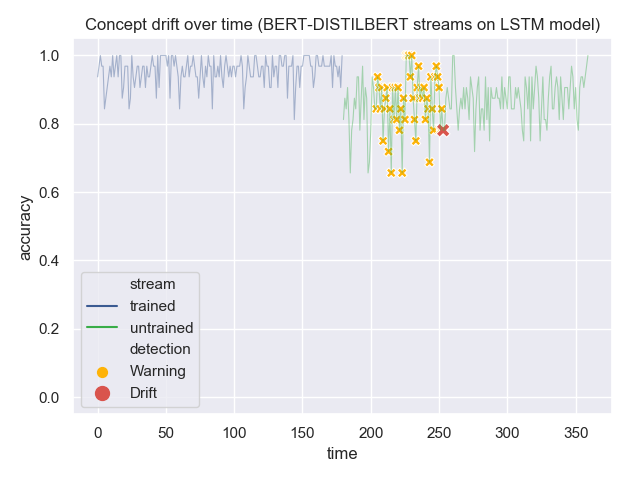
\includegraphics[width=\linewidth]{assets/detecting-change/diff_embed_lstm_wos_1_BERT_DISTILBERT.png}
  \caption{Supervised change detection}
  \label{fig:lstm-diff-embed-super-B-D}
\end{subfigure}%
\begin{subfigure}{.5\textwidth}
  \centering
  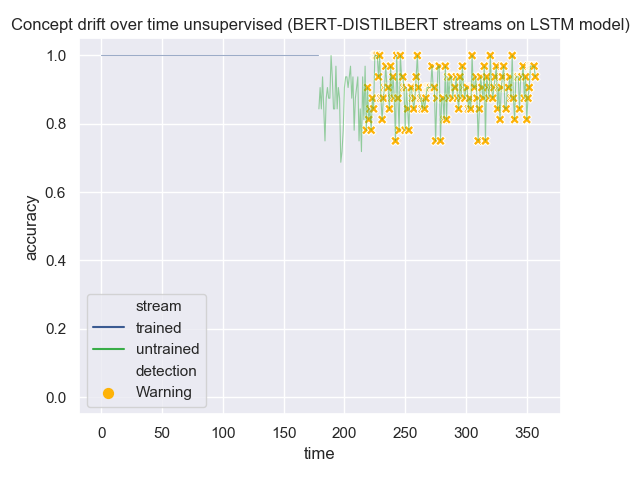
\includegraphics[width=\linewidth]{assets/detecting-change/diff_embed_lstm_wos_1_BERT_DISTILBERT_unsupervised.png}
  \caption{Unsupervised change detection}
  \label{fig:lstm-diff-embed-unsuper-B-D}
\end{subfigure}
\caption{Detecting change using different embeddings (BERT-DISTILBERT) in LSTM model}
\label{fig:lstm-diff-embed-B-D}
\end{figure}

Moving on to simulating big abrupt drift using a switch from BERT embeddings to DistilBERT, the results are showcased in figures \ref{fig:lstm-diff-embed-super-B-S} and \ref{fig:lstm-diff-embed-unsuper-B-S}. These results were again as expected, with a huge downgrade in the performance of the LSTM happening instantly since the SciBERT embedding space is very different from the BERT space. The change detector signals a drift immediately as well, outputting only two warnings in the supervised variant, and three in the unsupervised one. These is even faster than the results in the Naive Bayes model and this makes sense since the drop in performance is from almost perfect to random. The unsupervised case also performs exactly on par with the supervised, further proving that the method for detecting change when we have no labels works.

\begin{figure}[H]
\centering
\begin{subfigure}{.5\textwidth}
  \centering
  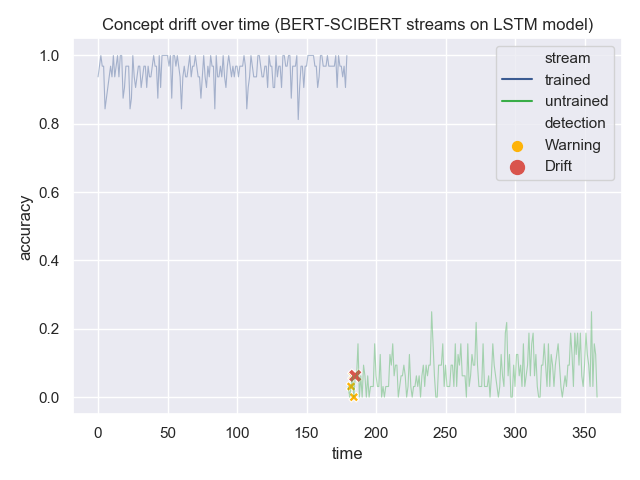
\includegraphics[width=\linewidth]{assets/detecting-change/diff_embed_lstm_wos_1_BERT_SCIBERT.png}
  \caption{Supervised change detection}
  \label{fig:lstm-diff-embed-super-B-S}
\end{subfigure}%
\begin{subfigure}{.5\textwidth}
  \centering
  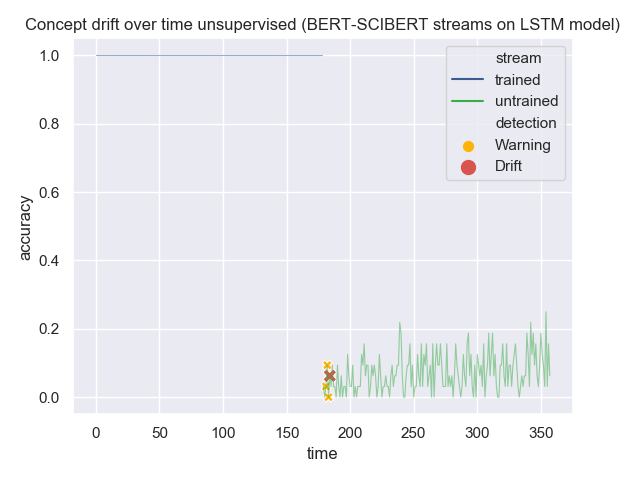
\includegraphics[width=\linewidth]{assets/detecting-change/diff_embed_lstm_wos_1_BERT_SCIBERT_unsupervised.png}
  \caption{Unsupervised change detection}
  \label{fig:lstm-diff-embed-unsuper-B-S}
\end{subfigure}
\caption{Detecting change using different embeddings (BERT-SCIBERT) in LSTM model}
\label{fig:lstm-diff-embed-B-S}
\end{figure}

Finally, figures \ref{fig:lstm-gradual-std-1}, \ref{fig:lstm-gradual-std-1}, and \ref{fig:lstm-gradual-std-1} present the results for adding gradual noise samples from a gaussian distribution with maximum standard deviations of $1.0$, $2.0$, and $3.0$ respectively to the BERT embeddings to simulate a gradual drift. These results again prove that the LSTM model is much more robust then the Naive Bayes one, because even when small random noise are added to the inputs that the model uses, it still retains its performance. This can be clearly seen in the figures, where for a maximum standard deviation of $1.0$, the model doesn't even have a performance drop for the whole duration of the stream, for a deviation of $2.0$, it only enters the warning zone towards the end of the stream with a drift being signalled right at the end, and for a deviation of $3.0$, the drift is detected after the middle of the stream.

\begin{figure}[H]
\centering
\begin{subfigure}{.5\textwidth}
  \centering
  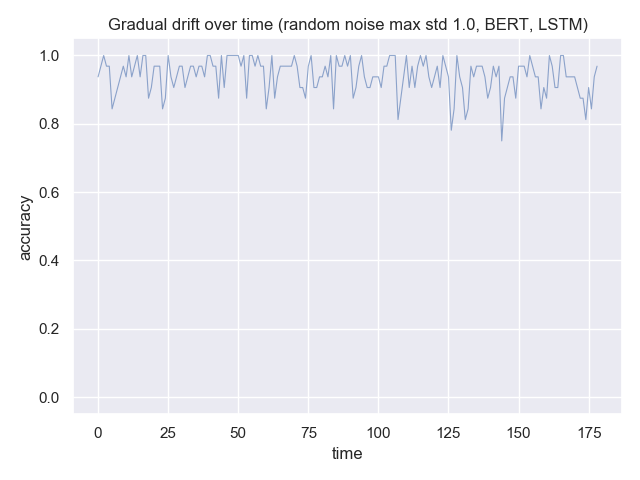
\includegraphics[width=\linewidth]{assets/detecting-change/gradual_noise_random_std_1_lstm_wos_1_BERT.png}
  \caption{Gradual with std 1.0}
  \label{fig:lstm-gradual-std-1}
\end{subfigure}%
\begin{subfigure}{.5\textwidth}
  \centering
  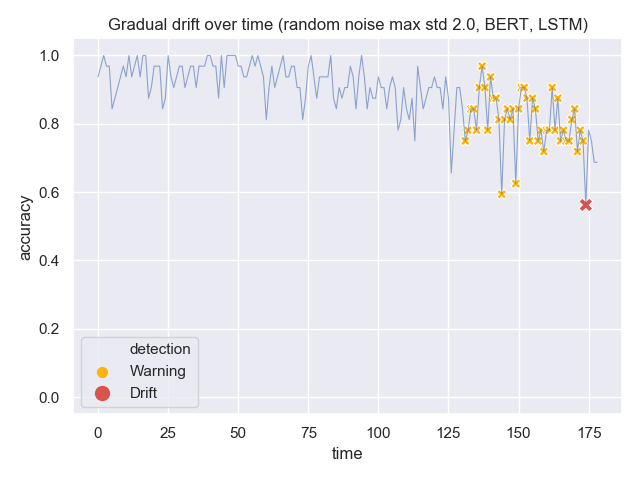
\includegraphics[width=\linewidth]{assets/detecting-change/gradual_noise_random_std_2_lstm_wos_1_BERT.png}
  \caption{Gradual with std 2.0}
  \label{fig:lstm-gradual-std-2}
\end{subfigure}
\begin{subfigure}{.5\textwidth}
  \centering
  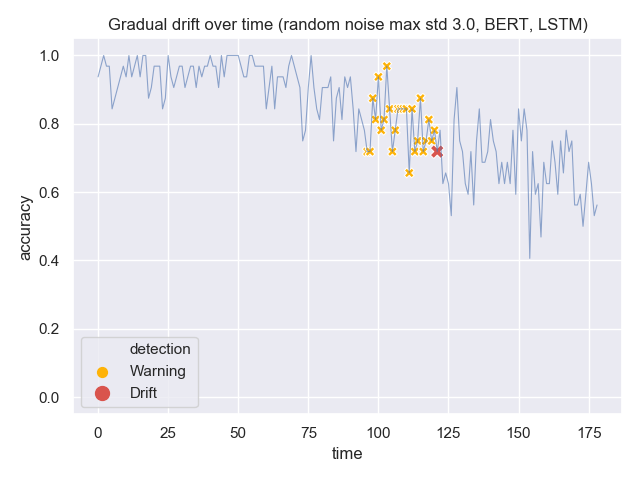
\includegraphics[width=\linewidth]{assets/detecting-change/gradual_noise_random_std_3_lstm_wos_1_BERT.png}
  \caption{Gradual with std 3.0}
  \label{fig:lstm-gradual-std-3}
\end{subfigure}
\caption{Detecting gradual change by adding random noise with different stds in the LSTM model}
\label{fig:lstm-gradual}
\end{figure}

\section{Discussion}

The results that were presented in the previous section showcase two important points:
\begin{itemize}
    \item There is a clear difference in robustness between the two models that we have chosen. The Naive Bayes model \emph{overfits} heavily on the dataset on which it was trained on, and thus any small perturbation in its input leads to a heavy degradation in the performance of the model. This can clearly be seen from the change to the DistilBERT embeddings, which are trained to be almost equivalent to the BERT ones, where the model performed much worse than expected. The LSTM, however, did not have these issues, only showing the expected slight degradation in its performance when switching to the DistilBERT embeddings.
    \item The second takeaway is that the change detectors work quite well for all the models and even when we don't have labels with which to compute the accuracies. The results in this chapter can be improved, however, if the user of the pipeline knows beforehand what type of change he expects. If gradual drift is expected, EDDM is the preferred method since it signals change faster than the normal DDM. For abrupt drift, DDM works very well in the supervised, while for the unsupervised case, it should be a little faster. If no labels are available, the sensitivity of the detector should be increased by decreasing the threshold for which a warning or a drift should be outputted.
\end{itemize}

\chapter{Addressing change} \label{sec:addressing}

After having solved the problem of detecting change in a data stream when the embeddings space is altered, this chapter now turns to addressing the issues caused by that change. Specifically, it attemps to answer the second research question outlined in the introduction (chapter \ref{sec:intro}), together with its two sub-questions: \emph{Given that a change was detected, how can we adapt the model efficiently such that the performance is the same as it previously was before the change?}. The work will be presented in the next two sections, with the first one focusing on addressing small abrupt drift, where we can probably recover the original accuracy just by fine-tuning the model with a few batches from the new embeddings space. The second section in this chapter focuses on the much harder task of adapting to big abrupt drift, where the idea is to find a mapping between the two embedding spaces.

It is also worth mentioning that since one of the big motivations of this thesis was to save both the time and the compute cost associated with training big neural network models, we will only be attempting to address the changes that happen to the LSTM model, not the Naive Bayes one. This is because the Naive Bayes model requires almost no time and computation cost to train, and so adapting it is just akin to retraining it from scratch.

\section{Fine-Tuning} \label{sec:fine}

Starting of with the first part of second research question: \emph{Given a small change (gradual drift or small abrupt drift), can we adapt the model by feeding it with a few examples, compared to retraining it from scratch?}, we address the small performance drop in the LSTM model (as seen in figure \ref{fig:lstm-diff-embed-B-D}) using a fine-tuning approach. Transfer learning has been an active area of research in deep learning for a few years now, keeping on trend with the need to make models cheaper and faster to train (\cite{survey-transfer-learning}). It is a technique that aims to exploit the knowledge gained in one type of problem on another related task or domain. Typically, the first layers of a neural network contain low level information about the task (such as edges or colors in the convolutional layers of a CNN according to \cite{survey-transfer-learning}), such that one can retrain only the last few layers of the network for the new task on which adaptation is required. This method is called fine-tuning, and altough it still requires some amount of learning, it is still much faster a full retrain.

Since the BERT and DistilBERT embeddings are so closely related by construction (\cite{distilbert}), we reckon we can use the fine-tuning approach in order to adapt the model from one embedding space to the other. \cite{fine-tuning-cd-image} mention that they use a similar approach to adapt an image dataset that suffers from concept drift for a classification task.

\subsection{Experimental Setup}

The approach taken to adapt the LSTM model to the DistilBERT embeddings is based on how convolutional neural networks are adapted to new datasets. Remember from section \ref{sec:lstm} that the architecture of the model was made out of two LSTM layers followed by a final fully connected layer that was used for classification. Since the LSTM layers learn the structure of text by determining the long term dependencies between the words (\cite{colahlstm}), we will keep these layers frozen, and only retrain the final classification layer. Since the fully connected layer only has a few parameters (2816 to be precise), the model can be adapted much faster than the time required to also retrain the two LSTM layers.

The experiments will take place in the same framework as those in the previous chapter, and they will have the same structure right before the adaptation part. We will start of with running the pipeline on the stream on which the model was trained on to build the statistics of the change detector, then we switch the embeddings while feeding the accuracies to the change detector and waiting for it to trigger warnings or drifts, and after the changed stream is finished, we finally move to the adaptation part. This final step of these experiments consist of re-running the stream with DistilBERT embeddings (this time with no change detector), and using the batches to train the classification layer of the LSTM while keeping track of the training accuracies to see if the model improves.

The adaptation part of the experiments will be run for 50, 100, and 200 batches to see how many are needed for the model to adapt properly. Moreover, the batches will be fed in random order as opposed to the other steps where the batches came in deterministically. This was to make sure that the model didn't see only batches that belonged to just a few classes, but actually receives a samples that are representative of the whole dataset.

\subsection{Results}

The results for the fine-tuning approach when switching from BERT to DistilBERT embeddings, thus creating a small drop in performance, are shown in figure \ref{fig:fine}. As mentioned above, we ran these experiments with three numbers of batches: 50, 100, and 200, which are shown in figures \ref{fig:fine50}, \ref{fig:fine100}, and \ref{fig:fine200} respectively. The figures show that, indeed, the fine-tuning approach manages to recover the accuracy of the model without needing to retrain the LSTM layers. While 50 seems to be too low of a number of batches for recovery, 100 already shows signs of clear improvement, while finally towards the end of the 200 batches it is quite clear that the performance of the model has recovered.

It is important to mention that the number of batches that need to be fed to the model in order for it to adapt is completely dependent on the actual model. While 200 batches work for this particular LSTM model, a different model may require a different number of batches. In most of the cases, however, fine-tuning should always manage to adapt the model quite fast, without needing to retrain from scratch.

\begin{figure}[H]
\centering
\begin{subfigure}{.48\textwidth}
\centering
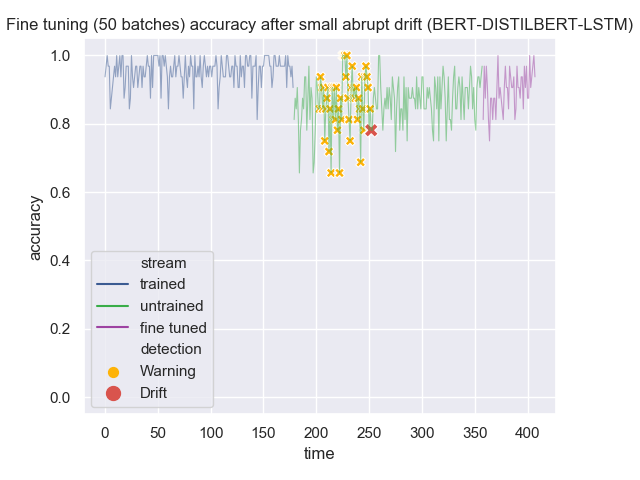
\includegraphics[width=\linewidth]{assets/addressing-change/fine_tuning_lstm_wos_1_BERT_DISTILBERT_50_batches.png}
\caption{Fine-tuning experiments using 50 batches}
\label{fig:fine50}
\end{subfigure}
\begin{subfigure}{.48\textwidth}
\centering
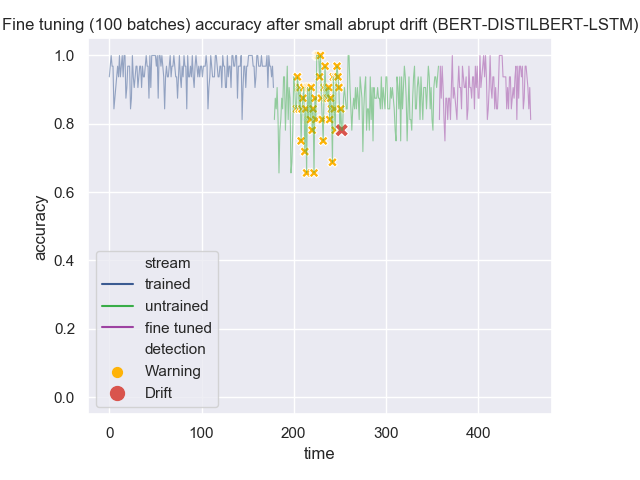
\includegraphics[width=\linewidth]{assets/addressing-change/fine_tuning_lstm_wos_1_BERT_DISTILBERT_100_batches.png}
\caption{Fine-tuning experiments using 100 batches}
\label{fig:fine100}
\end{subfigure}
\begin{subfigure}{.55\textwidth}
\centering
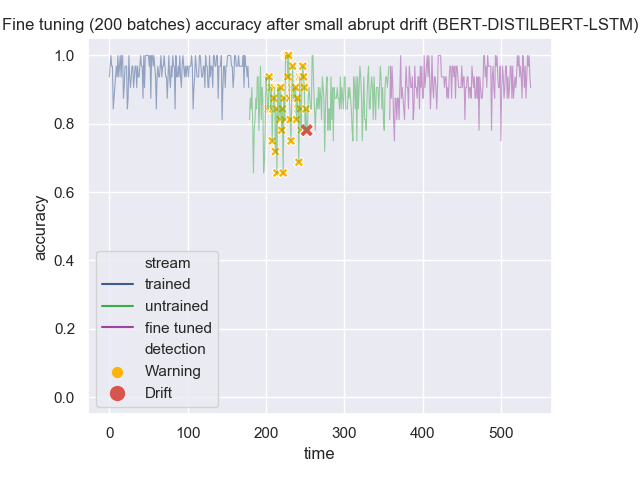
\includegraphics[width=\linewidth]{assets/addressing-change/fine_tuning_lstm_wos_1_BERT_DISTILBERT_200_batches.png}
\caption{Fine-tuning experiments using 200 batches}
\label{fig:fine200}
\end{subfigure}
\caption{Fine-tuning experiments}
\label{fig:fine}
\end{figure}

\cleardoublepage
\section{Mapping} \label{sec:map}

Part two of the second research question turns our attention to addressing a substantial drop in the performance of the model and answering the following: \emph{Given a big change (big abrupt drift), can we adapt the model by finding a mapping between the old outputs and the new ones which is less expensive to compute than retraining the model from scratch?}. As mentioned in the question above, this complicated problem will be approached by trying to find a mapping from the new embeddings (SciBERT) to the old ones (BERT), thus keeping the model trained on the BERT embeddings frozen and adding a new component to our framework \ref{fig:framework} through which all inputs will be going through such that they are switched from SciBERT to BERT so the model can understand them.

The Natural Language Processing field has been studying this mapping idea for a few years now, but in the different context of trying to learn cross-lingual word embeddings. These methods attempt to find a mapping between embeddings for a source language and embeddings for a target language such that a model trained on the source languge embeddings can also work with inputs that come from the target language. \cite{mikolov2013distributed} first suggested this approach as an extension to their seminal \textbf{word2vec} paper (\cite{word2vec}), in which they contruct a parallel corpus of words, each with a representation in the source embeddings space and the target embeddings space. The source matrix will be denoted as $S$, while the target matrix as $T$. They found that learning a simple linear mapping between $S$ and $T$ achieves similar results to more complicated solutions such as a multilayer neural network. Both \cite{normalized-word-embbedings} and \cite{principle-bilingual-mappings} then found that enforcing an orthogonality constraint on the mapping matrix achieves better results on the same tasks. By putting this constraint in the problem, we transform it to the Orthogonal Procrustes problem (\cite{procrustes}). This states that given two matrices $S$ and $T$, we would like to find a orthogonal matrix $M$ that maps $S$ to $T$ as closely as possible. This boils down to the following equation:

\begin{equation}
    M = \argmin_{M'} ||M' S - T ||_F
\end{equation}
, where $M'^T M' = I$. The closed-form solution can be found using Singular Value Decomposition on the matrix product between $T$ and $S^T$, such that $U\Sigma V^T = \text{SVD}(TS^T)$ and $M = UV^T$. Both of the papers mentioned above rely on the assumption that there are bilingual dictionaries or parallel corpora readily available. The MUSE framework (\cite{muse}) manages to overcome this issue by employing a GAN (\cite{gan}) to train the mapping, where the generator acts as the actual mapping and the discriminator tries to guess whether a sample comes from the actual target embeddings or the mapped ones. The generator is then used a means to construct the bilingual dictionary which can finally be used to construct the linear mapping. This method manages to achieve results that are comparable with the Procrustes mapping when parallel data is actually available.

What all these methods described above have in common is that they assume that the embeddings used are non-contextualized (e.g., word2vec, glvoe), meaning that they only output one vector of embeddings per each word in the text, making it quite straightforward to construct a one to one mapping between the source and target embeddings. This is contrary to contextualized embeddings (e.g., BERT, ELMo), which can output multiple tokens per word thus producing multiple embedding vectors. Take for example the word \emph{contextualized}. Its token representation when using BERT is $\begin{bmatrix} 101 & 6123 & 8787 & 3550 & 102 \end{bmatrix}$, while its representation when using SciBERT is $\begin{bmatrix} 102 & 11695 & 645 & 103 \end{bmatrix}$, and all these tokens have their respective vector representation. As we can see, both the number of tokens is different and also the tokens do not correspond between the two representations, thus it is impossible to construct a one to one mapping between the words in this manner. Both \cite{crosslingual} and \cite{investigating-cross-lingual} have recently explored this problem in their work, but again in the context of trying to learn cross-lingual contextualized word embeddings. They define a word anchor as the aggregated representation of all the tokens in the word, where an aggregation can be either the average or the maximum of the token embeddings. They argue that a mapping learned using the anchors should hopefully generalize to the token-level embeddings as well. \cite{crosslingual} arrive at this conclusion because they plotted the token representations of a few different words and found that the tokens for a word tend to cluster together in a point cloud.

\subsection{Experimental Setup}

Having given the necessary background into mappings between different embedding spaces, we can now explain how we are going to run our experiments. Before even talking about mappings we first need construct a suitable dataset from our existing one, since token-level embeddings cannot be aligned, as explained above. Thus, we have decided to look through the whole Web of Science dataset and find the most common 5000 or 10000 words there since picking all the words might skew the mapping because of noise. Then for all of the picked words, we can use both BERT and SciBERT to tokenize and subsequently embed them. Finally, we use the two aggregation methods described above (namely the maximum and the average) to get one embeddings representation per word resulting in the parallel dataset on which we can train a mapping.

Two methods will be tried in our experiments. The first is the classic Procrustes linear mapping, where the source matrix will be the SciBERT embeddings and the target matrix the BERT embeddings, both of them for the most common 5000 words. We expect this mapping to be very fast to train since it's a simple SVD on a matrix product, but not a very accurate mapping because it's linear, thus inflexible. The second mapping that we picked was a simple multilayer perceptron with two fully connected layers that sandwich a ReLU activation function, such that the mapping is non-linear. We expect this one to be a little slower to train because even though it's a small network it still is a neural network trained using gradient descent, but it should be more flexible than the linear mapping.

We will put these assumptions to test in two ways. First, we want to measure how well the source matrix is actually mapped to the target and so we will showcase this by computing the mean-squared error between the mapped source matrix and the target and visualizing the embedding spaces using both PCA (\cite{pca}) and t-SNE (\cite{tsne}). Second, we also have to check how these mappings actually translate to a potential recovery in the performance of the LSTM model. For this purpose, we again turn to our pipeline to run the Web of Science stream three times: first, using the data transformed using BERT to build the statistics of the change detector, then we change the embeddings to SciBERT and let the detector do its work, and finally we again run the SciBERT stream but this time mapped to the BERT space using either the linear or the non-linear mapping.

Finally, we note that the linear mapping will be trained on the most common 5000 words, while the non-linear mapping will be trained on the most common 10000 since the MLP needs more training data.

\subsection{Results}

We first present the results for the linear Procrustes mapping. As assumed, it was trained very fast, in just 2.34 seconds, on the 5000 most common words parallel dataset. Before the mapping, the MSE score between the source and the target is equal to $0.7274$. After mapping, that score is reduced to $0.3134$, which is quite good for an inflexible linear mapping, but still far from a robust mapping. This can also be seen from the PCA (figure \ref{fig:proc-pca}) and the t-SNE (figure \ref{fig:proc-tsne}) visualizations. The red points in the visualizations are the source (SciBERT) embeddings, the green points are the target embeddings (BERT), and finally the blue ones are the mapped embeddings. If the mapping was perfect, the green and blue point clouds should be the same, but as we can see from figures, the point clouds are still pretty far from each other.

\begin{figure}[H]
\centering
\begin{subfigure}{.49\textwidth}
\centering
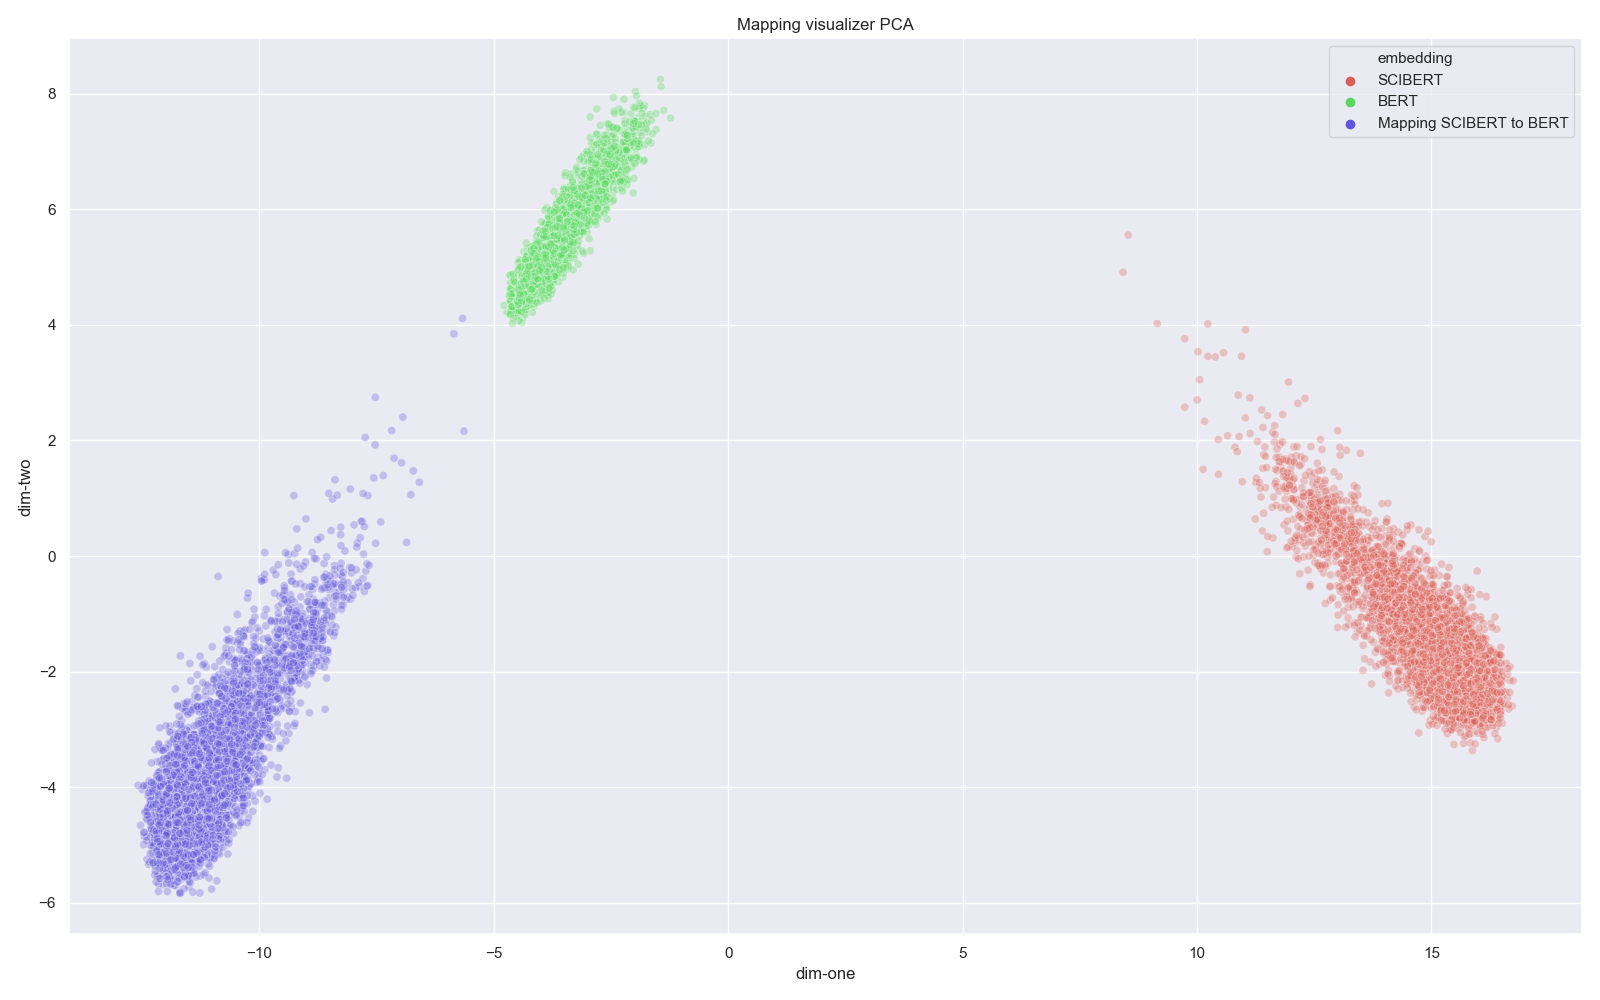
\includegraphics[width=\linewidth]{assets/addressing-change/mapping_vis_pca_SCIBERT_BERT_average.png}
\caption{Visualization using PCA}
\label{fig:proc-pca}
\end{subfigure}
\begin{subfigure}{.49\textwidth}
\centering
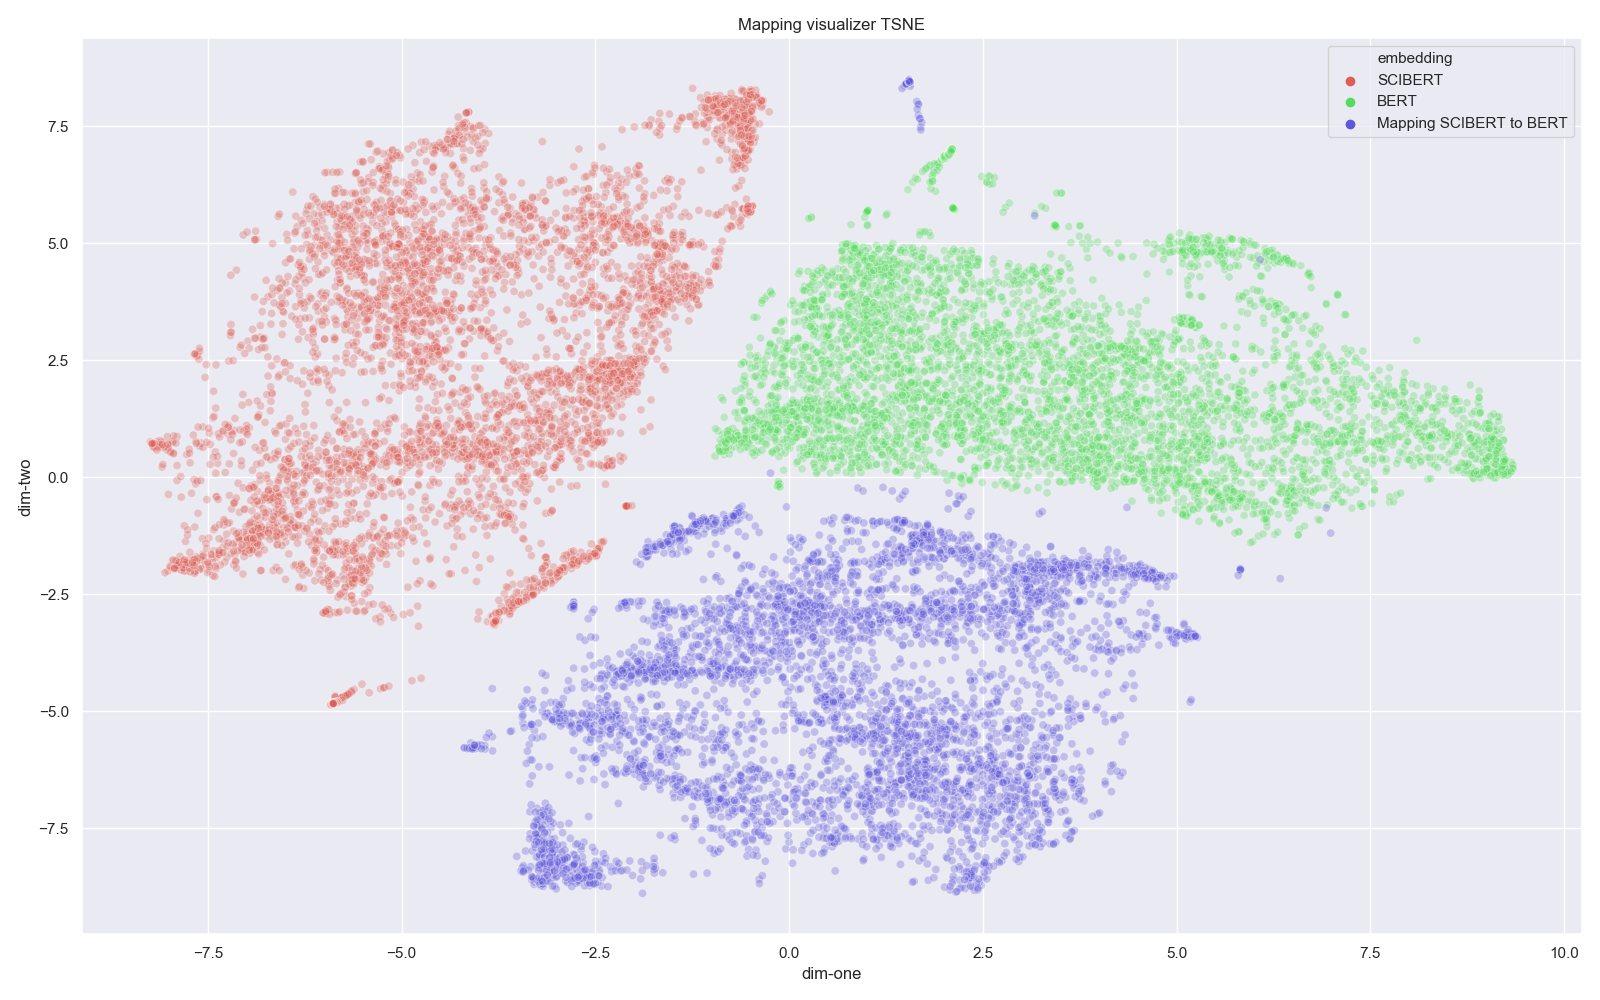
\includegraphics[width=\linewidth]{assets/addressing-change/mapping_vis_tsne_SCIBERT_BERT_average.png}
\caption{Visualization using t-SNE}
\label{fig:proc-tsne}
\end{subfigure}
\caption{Visualizations for BERT, SciBERT, and the mapping between the two done using Procrustes}
\label{fig:proc-viz}
\end{figure}

However, the Procrustes mapping still yields a decent improvement in the performance of the model, as can be seen from figure \ref{fig:proc-results}. The mapping manages to achieve a decent average of 0.43 accuracy with a few outliers that also reach the performance of the model with the initial embeddings.The results are quite similar when using either the maximum or the average aggregation menthods, with the maximum slightly outperforming the average.

\begin{figure}[H]
\centering
\begin{subfigure}{.49\textwidth}
\centering
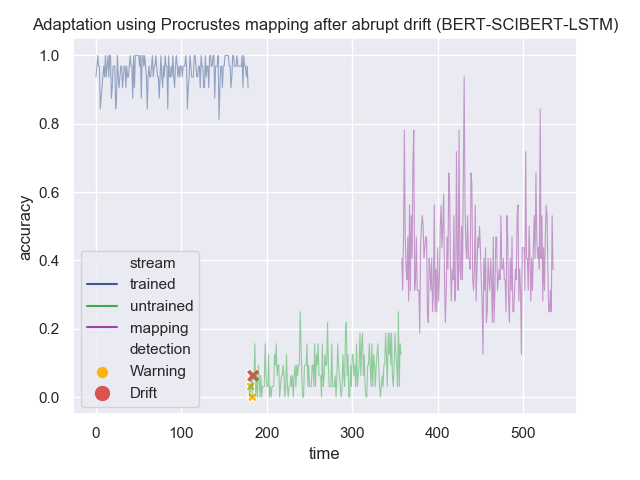
\includegraphics[width=\linewidth]{assets/addressing-change/procrustes_lstm_wos_1_BERT_SCIBERT_5000_words_max.png}
\caption{Results using \textbf{max} embeddings aggregation in the dataset}
\label{fig:proc-max}
\end{subfigure}
\begin{subfigure}{.49\textwidth}
\centering
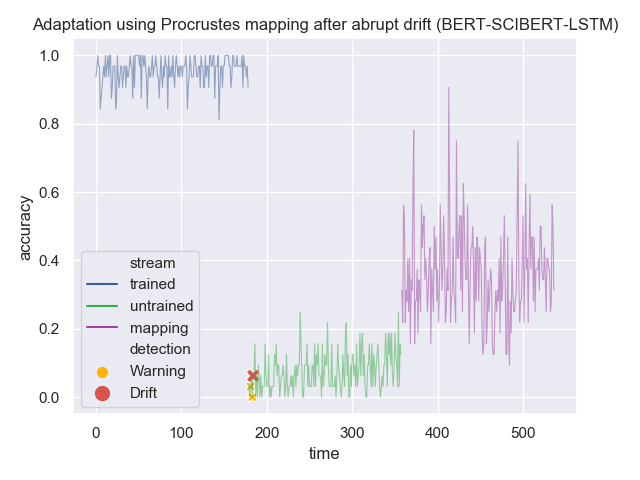
\includegraphics[width=\linewidth]{assets/addressing-change/procrustes_lstm_wos_1_BERT_SCIBERT_5000_words_average.png}
\caption{Results using \textbf{average} embeddings aggregation in the dataset}
\label{fig:proc-average}
\end{subfigure}
\caption{Results for adaptation using the Procrustes mapping}
\label{fig:proc-results}
\end{figure}

Moving on to the MLP mapping, we can see from figures \ref{fig:mlp-pca} and \ref{fig:mlp-tsne} that the BERT embeddings represented by the green point cloud and the mapped embeddings represented by the blue point cloud overlap substantially, which is to be expected since we introduced a non-linearity between the two fully connected layers that reduces the bias of the model. This is verified by the MSE scores, with a $0.7205$ before the mapping and a $0.1149$ after. The training time is much longer than the linear mapping, with 31.76 seconds, but which is still much quicker than a full retraining of the model.

The full summary for the scores and training times can be seen in table \ref{table:maps}.

\begin{figure}[H]
\centering
\begin{subfigure}{.49\textwidth}
\centering
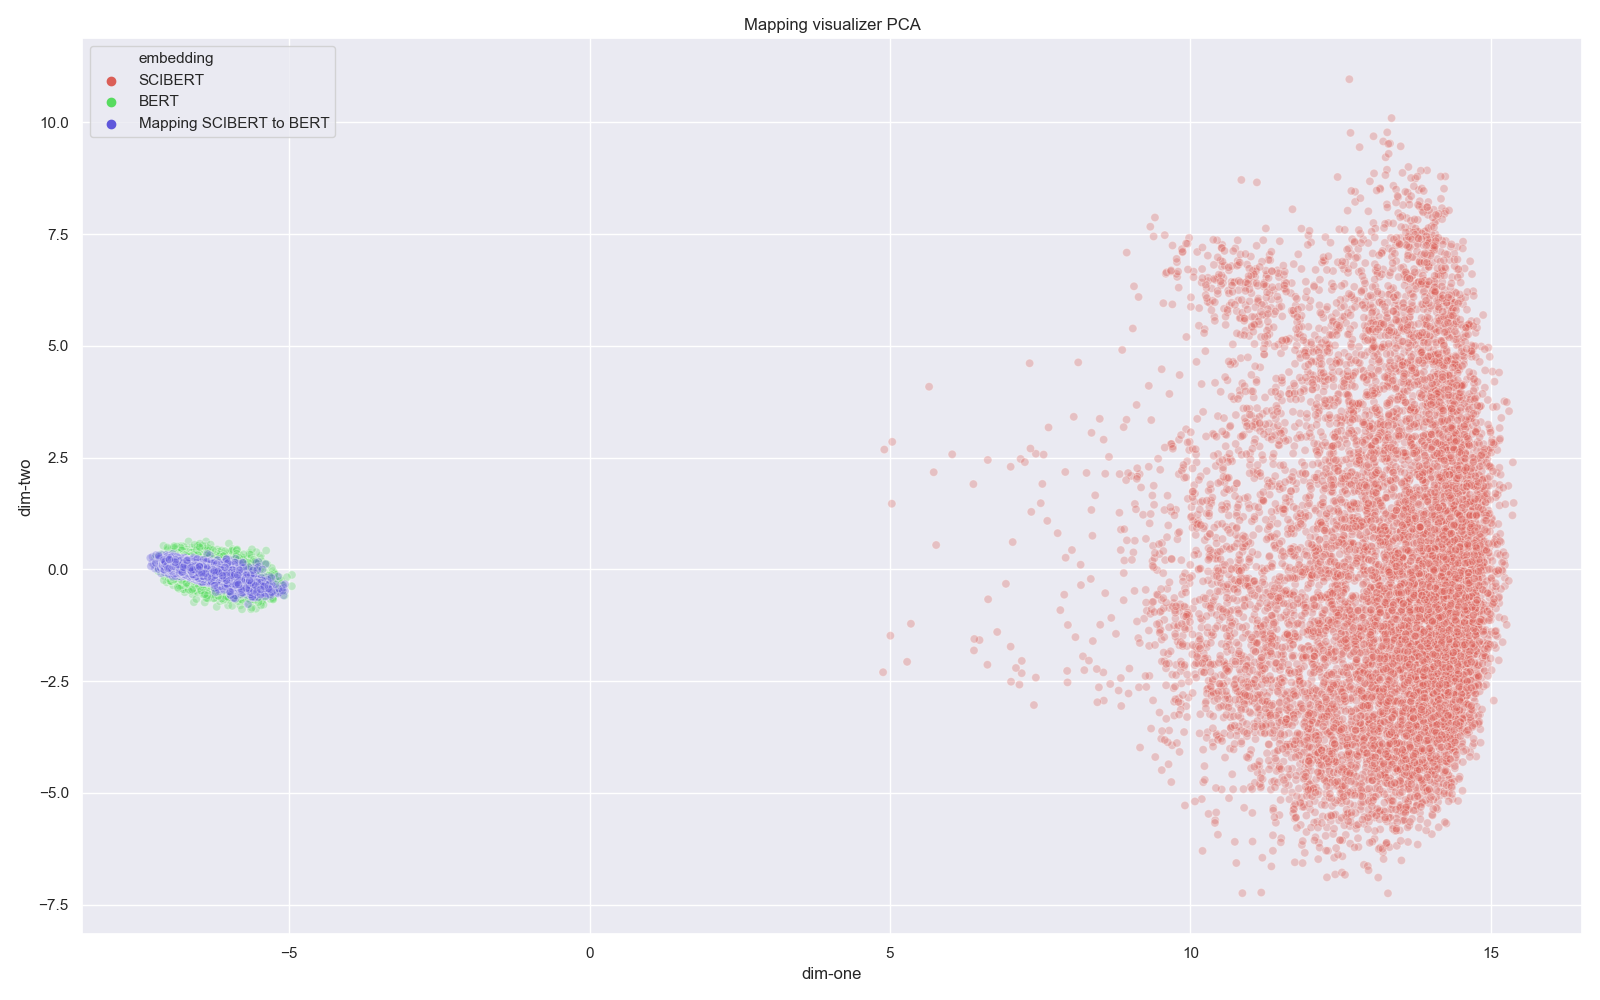
\includegraphics[width=\linewidth]{assets/addressing-change/mlp_mapping_vis_pca_SCIBERT_BERT_average.png}
\caption{Visualization using PCA}
\label{fig:mlp-pca}
\end{subfigure}
\begin{subfigure}{.49\textwidth}
\centering
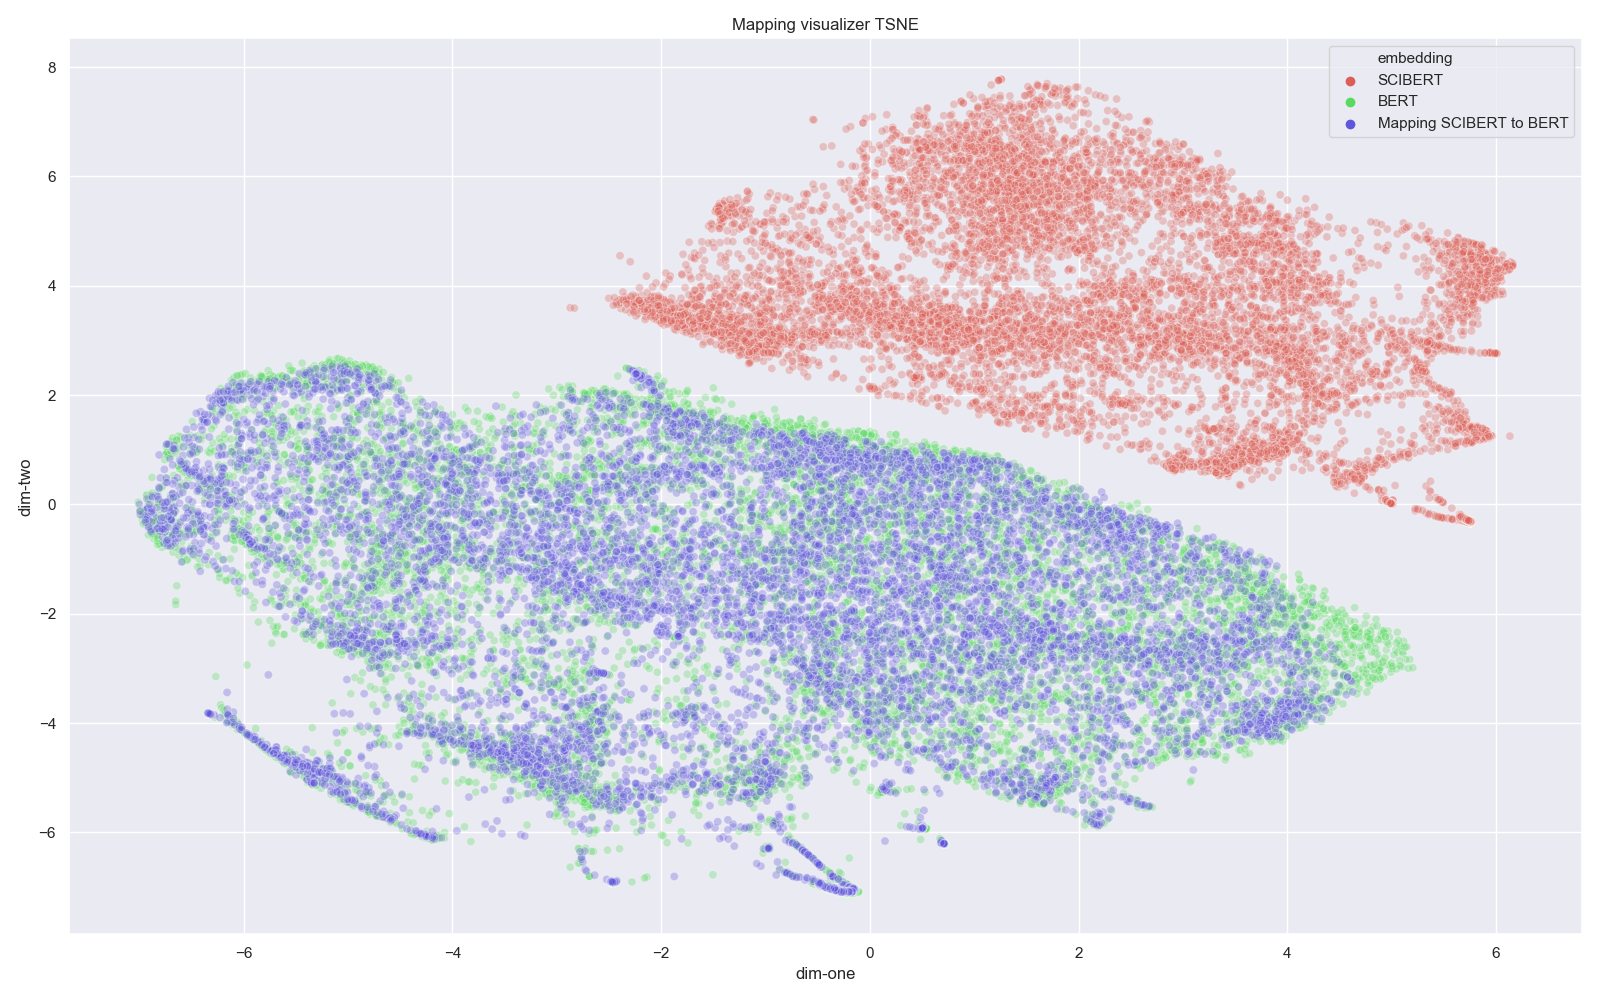
\includegraphics[width=\linewidth]{assets/addressing-change/mlp_mapping_vis_tsne_SCIBERT_BERT_average.png}
\caption{Visualization using t-SNE}
\label{fig:mlp-tsne}
\end{subfigure}
\caption{Visualizations for BERT, SciBERT, and the mapping between them done using MLP}
\label{fig:mlp-viz}
\end{figure}

Even though the MLP mapping manages to make the two point clouds of our dataset overlap, this however doesn't translate to good performance on our adaptation task. As can be seen from figure \ref{fig:mlp-results}, there is some accuracy improvement compared to the non-mapped stream, but it is small, and more importantly, it performs worse than the linear mapping. There is also a clear difference between the two aggregation methods here, with the average one performing better than the max one. These figures also contain a few outliers, suggesting that some tokens are mapped well.

\begin{figure}[H]
\centering
\begin{subfigure}{.49\textwidth}
\centering
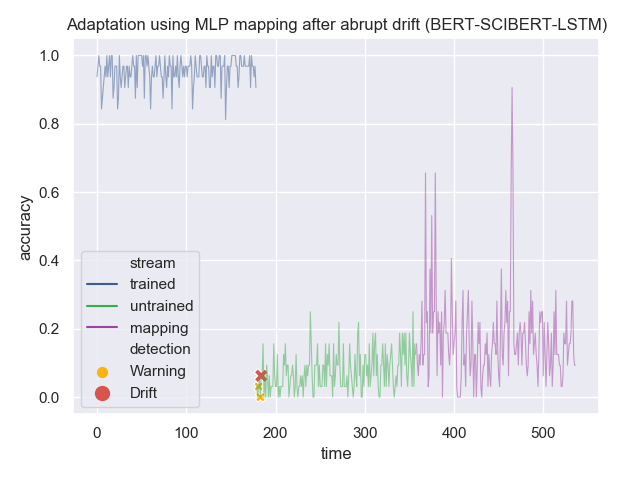
\includegraphics[width=\linewidth]{assets/addressing-change/mlp_mapping_lstm_wos_1_BERT_SCIBERT_10000_words_max.png}
\caption{Results using \textbf{max} embeddings aggregation in the dataset}
\label{fig:mlp-max}
\end{subfigure}
\begin{subfigure}{.49\textwidth}
\centering
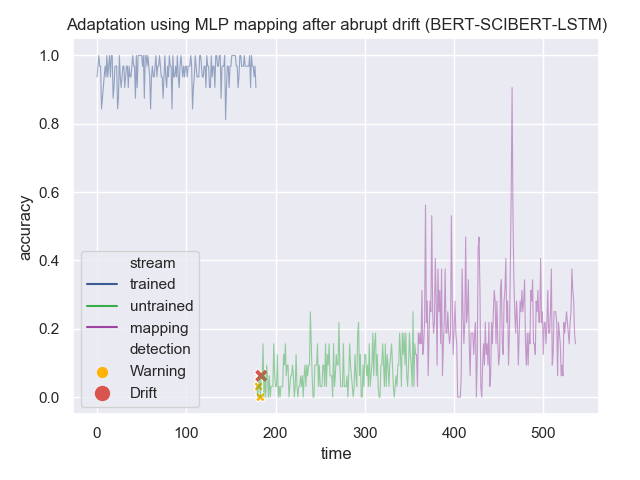
\includegraphics[width=\linewidth]{assets/addressing-change/mlp_mapping_lstm_wos_1_BERT_SCIBERT_10000_words_average.png}
\caption{Results using \textbf{average} embeddings aggregation in the dataset}
\label{fig:mlp-average}
\end{subfigure}
\caption{Results for adaptation using the MLP mapping}
\label{fig:mlp-results}
\end{figure}

\begin{table}[H]
\centering
\begin{tabular}{|l|l|l|l|}
\hline
                  & MSE before mapping & MSE after mapping & Train time \\ \hline
Procrustes (5000 words) & 0.7274             & 0.3134            & 2.34s      \\ \hline
MLP (10000 words)       & 0.7205             & 0.1149            & 31.76s     \\ \hline
\end{tabular}
\caption{MSE scores and training times for both the Procrustes and the MLP mappings}
\label{table:maps}
\end{table}

\section{Discussion}

We can conclude from section \ref{sec:fine} that the first part of the second research question is answered by the fine-tuning approach to adapt from small abrupt concept drift. This approach can also be used to adapt from gradual drift by just using every sample to fine-tune the model continuously throughout the runtime of the pipeline, as mentioned in \cite{fine-tuning-cd-image}. The fine-tuning can be triggered automatically whenever the model enters the warning zone, because if it is started only after a drift, the model might have diverged too far for a fine-tuning approach to work (as seen in figures \ref{fig:lstm-gradual-std-2} and \ref{fig:lstm-gradual-std-3}).

As for the second part of that research question, we believe that the Procrustes mapping performs as well as it can given its linear narute, but the MLP mapping presents quite a paradox. On one hand, it maps the dataset that we contructed well, but on the other hand, it doesn't manage to adapt the model to the new embeddings SciBERT embeddings. We believe that this happens because of how we contructed the dataset using the anchors. Since the MLP is non-linear, it manages to contruct a mapping with a low MSE score but that means that it also doesn't generalize to the non-anchored dataset which is used in the LSTM model. The Procrustes method on the other hand doesn't have such a low MSE score, but this translates to less overfitting on our anchored dataset and more generalization on the initial on. We have trained to fix this generalization problem by adding a dropout layer (\cite{dropout}) to the MLP for less overfitting, but that did not fix the issues. We also believe that a more complex neural network model would not help here since the issue isn't about the flexibility of the model, but about the dataset. Thus, we conclude that the second part of the adaptation research question is not answered for now and we discuss a few ideas for future work in chapter \ref{sec:conclusion}.

\chapter{Prototype Implementation} \label{sec:prototype}

\chapter{Conclusion and Future Work} \label{sec:conclusion}

\addcontentsline{toc}{chapter}{Bibliography}
\setcitestyle{numbers}
\bibliographystyle{plainnat}
\bibliography{references.bib}

\end{document}

